% ============================================================
%  ch05_teff.tex — Nonlinear Effective Temperature Formalism
%  Requires: macros.tex, amsmath, amssymb, amsthm
%  Estimated length: 20–28 pages
%  Rewritten: VD-08, 2026-03-07
% ============================================================

\chapter{Nonlinear Effective Temperature Corrections}
\label{ch:teff}

The MES bounds of Chapter~\ref{ch:bianchi-bounds} operate in the
linearised regime, where the CMB temperature field is expanded to
first order in the kinematic variables.  The effective temperature
formalism, developed by Maartens, Gebbie \&
Ellis~\cite{MaartensGE1999}, provides a nonlinear generalisation:
the exact photon distribution function is integrated over energy
to yield an angle-dependent effective temperature $\Teff(\mathbf{e})$
whose fourth power gives the bolometric intensity.  The moment map
of $\Teff^4$ over the sky sphere encodes the nonlinear coupling
between multipoles and provides corrections to the linearised bounds
that, at the dipole-anomaly amplitude, reach $\sim 0.8\%$ for the
shear at S3 (rising to $\sim 1.8\%$ at the S2c radio-dipole
amplitude)---not negligible for precision work.

Our goal in this chapter is to build the complete $\Teff$ formalism
from the covariant Boltzmann equation, extend the existing
shear-only moment map to include vorticity and four-acceleration as
primary source terms, derive the $\ell$-pole mixing matrix, analyse
the Einstein--$\Teff$ ODE system, and synthesise the comprehensive
nonlinear corrections.  The presentation follows the VN-series
analyses (VN-01 through VN-05) and constitutes, to our knowledge,
the first unified treatment of all four kinematic contributions to
the nonlinear $\Teff$ formalism.


% ============================================================
\section{The covariant Boltzmann equation}\label{sec:boltzmann-eq}
% ============================================================

\subsection{Phase-space decomposition}\label{sec:phase-space}

Before diving into the multipole hierarchy, we establish the
Boltzmann equation in the 1+3 covariant framework.  A photon
with four-momentum $p^a$ decomposes relative to the fundamental
observer $u^a$ as
\begin{equation}\label{eq:photon-decomp}
p^a = E\,(u^a + e^a)\,,
\end{equation}
where $E = -p_a u^a$ is the photon energy measured by $u^a$ and
$e^a$ is the spatial propagation direction ($e_a u^a = 0$,
$e_a e^a = 1$).  The photon distribution function
$f(x^a, E, e^a)$ satisfies the Boltzmann equation
\begin{equation}\label{eq:boltzmann}
L[f] = C[f]\,,
\end{equation}
where $L$ is the Liouville operator (free streaming along null
geodesics) and $C$ is the collision operator (Thomson
scattering).


\subsection{The Liouville operator}\label{sec:liouville}

The Liouville operator in the 1+3 decomposition takes the
form~\cite{EllisVanElst1999,MaartensGE1999}
\begin{equation}\label{eq:liouville}
\begin{split}
L[f] &= E\,\frac{\partial f}{\partial t}
  + e^a\,\tilde{D}_a f
  - E\,\frac{\partial f}{\partial E}\bigl[
    \tfrac{1}{3}\Theta + \sigma_{ab}\,e^a e^b
    + \dot{u}_a\,e^a
  \bigr] \\
  &\quad + E\,\frac{\partial f}{\partial e^a}\bigl[
    \dot{u}^a + \tfrac{1}{3}\Theta\,e^a
    + (\sigma^a{}_b + \omega^a{}_b)\,e^b
    - (\sigma_{cd}\,e^c e^d)\,e^a
  \bigr]\,,
\end{split}
\end{equation}
where $\partial/\partial t = u^a \nabla_a$ is the covariant
time derivative.  Two structural features are evident from
Eq.~\eqref{eq:liouville}:

(a) The energy derivative $\partial f/\partial E$ contains
$\Theta$ (isotropic redshift), $\sigma_{ab}e^a e^b$ (anisotropic
redshift from shear), and $\dot{u}_a e^a$ (gravitational
redshift from acceleration).  Vorticity does \emph{not} appear
in the energy equation because $\omega_{ab}e^a e^b = 0$ by
antisymmetry.

(b) The direction derivative $\partial f/\partial e^a$ contains
$\omega^a{}_b e^b$ (frame dragging from vorticity) and the shear
and acceleration terms.  Vorticity enters exclusively through
the rotation of the photon propagation direction, not through
energy shifts.


\subsection{The collision operator}\label{sec:collision}

Thomson scattering of photons off electrons gives the collision
term
\begin{equation}\label{eq:thomson}
C[f] = n_e\,\sigma_T\,E\Bigl[
  -f + f_0\bigl(1 + e^a v_a^{(e)}\bigr)
\Bigr]\,,
\end{equation}
where $n_e$ is the free electron number density, $\sigma_T$ is
the Thomson cross section, $f_0$ is the isotropic equilibrium
distribution, and $v_a^{(e)}$ is the electron bulk velocity.
In the tight-coupling regime ($n_e\sigma_T \gg H$), the
collision term forces the photon distribution to be nearly
isotropic in the electron rest frame, with a residual dipole
tracking the baryon velocity.  After decoupling, $C[f] = 0$
and the photons free-stream.


% ============================================================
\section{The PSTF multipole hierarchy}\label{sec:pstf-hierarchy}
% ============================================================

\subsection{Energy-integrated multipoles}\label{sec:energy-int}

The energy-integrated intensity multipoles are defined by
\begin{equation}\label{eq:I-multipole}
I_{A_\ell}(x)
= \int_0^\infty E^3\,f(x, E, e)\,
  e^{\langle a_1}\cdots e^{a_\ell\rangle}\,dE\,d\Omega_e\,,
\end{equation}
where $d\Omega_e$ is the solid angle element on the unit sphere
of directions and angle brackets denote the PSTF projection.
The monopole $I$ is proportional to the radiation energy density
($I \propto \rho_\gamma \propto T^4$), the dipole $I_a$ to the
radiation energy flux, and the quadrupole $I_{ab}$ to the
radiation anisotropic stress.


\subsection{Multipole divergence equations}
\label{sec:MDE}

Integrating the Boltzmann equation~\eqref{eq:boltzmann} against
$E^3 e^{\langle A_\ell\rangle}$ and performing the angular
integrals yields the multipole divergence equations
(MDEs)~\cite{MaartensGE1999,ChallinorLasenby1999}.  The general
form is
\begin{equation}\label{eq:MDE-general-teff}
\dot{I}_{A_\ell}
+ \tfrac{4}{3}\Theta\,I_{A_\ell}
+ \tilde{D}^b I_{bA_\ell}
- \frac{\ell}{2\ell+1}\,\tilde{D}_{\langle a_\ell}
  I_{A_{\ell-1}\rangle}
+ \tfrac{4}{3}\,I\,\dot{u}_{a_1}\,\delta_{\ell 1}
- \tfrac{8}{15}\,I\,\sigma_{a_1 a_2}\,\delta_{\ell 2}
= \mathcal{C}_{A_\ell}\,,
\end{equation}
where $\mathcal{C}_{A_\ell}$ contains the Thomson scattering
terms.  The explicit transport equations for
$\ell = 0, 1, 2, 3$ were given in
Eqs.~\eqref{eq:ell0}--\eqref{eq:ell3} of
Chapter~\ref{ch:bianchi-bounds}.


\subsection{The $\ell$-pole coupling structure}
\label{sec:ell-coupling}

The coupling pattern of the four kinematic quantities in the
MDE hierarchy determines the nonlinear mixing structure that
the $\Teff$ formalism captures.  We summarise the couplings:

\emph{Expansion} $\Theta$: diagonal in $\ell$, scaling each
multipole as $\frac{4}{3}\Theta\,I_{A_\ell}$.  The expansion
dilutes all multipoles uniformly and does not mix different
$\ell$ values.

\emph{Shear} $\sigma_{ab}$: enters as a source in the
$\ell = 2$ equation with coefficient $8/15$.  Through the
nonlinear terms (products of multipoles in the exact Boltzmann
equation), the shear induces $\Delta\ell = \pm 2$ mixing:
$\ell = 0 \leftrightarrow 2$,
$\ell = 1 \leftrightarrow 3$, etc.  The mixing coefficient is
proportional to the Wigner $3j$-symbol
$\bigl(\begin{smallmatrix} \ell & 2 & \ell' \\
0 & 0 & 0 \end{smallmatrix}\bigr)$.

\emph{Vorticity} $\omega_{ab}$: does not appear in the energy
equation (because $\omega_{ab}e^a e^b = 0$) but enters through
the direction equation.  At the nonlinear level, vorticity
generates $\Delta\ell = \pm 1$ mixing through the
$\varepsilon_{abc}$-structure:
$\ell = 0 \leftrightarrow 1$,
$\ell = 1 \leftrightarrow 2$, etc.  The mixing has
\emph{odd parity} ($(-1)^{\ell+1}$ under spatial inversion),
distinguishing it from all other kinematic contributions.

\emph{Acceleration} $\dot{u}_a$: enters the $\ell = 1$
equation with coefficient $4/3$.  At the nonlinear level,
acceleration generates $\Delta\ell = \pm 1$ mixing through the
$\dot{u}_{\langle a_\ell}I_{A_{\ell-1}\rangle}$ coupling, with
\emph{even parity}.  The even-parity character means that the
acceleration mixing is \emph{coherent} with the shear pattern
(both are $m = 0$ for axisymmetric models), while the vorticity
mixing is \emph{orthogonal}.

The leading-order coefficients for each mixing channel are:
\begin{equation}\label{eq:mixing-coefficients}
\begin{aligned}
\text{shear:}\quad &
  c_{\ell,\ell+2}^{(\sigma)}
  = -\frac{8}{15}\,
    \frac{(\ell+1)(\ell+2)}{(2\ell+1)(2\ell+3)}\,,\\[3pt]
\text{vorticity:}\quad &
  c_{\ell,\ell+1}^{(\omega)}
  = \frac{\ell+1}{2\ell+3}\,
    |\omega|/\Theta\,,\\[3pt]
\text{acceleration:}\quad &
  c_{\ell,\ell+1}^{(\dot{u})}
  = \frac{4}{3}\,
    \frac{|\dot{u}|/\Theta}{2\ell+1}\,\delta_{\ell 0}\,.
\end{aligned}
\end{equation}
The acceleration coupling is sharply localised to $\ell = 0
\leftrightarrow 1$ (it appears only in the dipole equation),
while the vorticity coupling extends to all $\ell$.
Figure~\ref{fig:ell_mixing_comparison} plots the leading-order
boost mixing coefficients as functions of $\beta$, confirming that
the $\ell = 2 \to 1$ channel dominates at $O(\beta)$ while the
$\ell = 2 \to 0$ channel enters only at $O(\beta^2)$.


% ============================================================
\section{The $\Teff$ ansatz}\label{sec:teff-ansatz}
% ============================================================

\subsection{Motivation: truncation versus representation}
\label{sec:trunc-rep}

The MDE hierarchy~\eqref{eq:MDE-general-teff} is an infinite coupled
system: each $\ell$ equation involves $I_{A_{\ell+1}}$ through
the gradient term, creating an unbounded chain.  Standard
approaches truncate the hierarchy at some $\ell_{\mathrm{max}}$
and close the system by setting
$I_{A_{\ell_{\mathrm{max}}+1}} = 0$ (or by a more sophisticated
closure scheme).  The accuracy of the result depends on
$\ell_{\mathrm{max}}$ and on the physics that drives power to
high multipoles.

The $\Teff$ approach takes a fundamentally different strategy.
We do \emph{not} close the hierarchy algebraically.  Instead,
we parameterise the full angular temperature field by a
finite-dimensional manifold of shapes and \emph{monitor
tangency}: we check whether the exact solution remains tangent
to the parameterised manifold within controlled error bounds.
The distinction is between truncation (which discards
information) and representation (which projects the full
solution onto a finite basis and tracks the residual).


\subsection{The normalised temperature field}
\label{sec:Theta-field}

We define the normalised effective temperature
\begin{equation}\label{eq:Theta-def}
\Theta(\mathbf{e}) := \frac{\Teff(\mathbf{e})}{T_0}\,,
\end{equation}
where $T_0 = \langle\Teff\rangle_\Omega$ is the monopole
temperature.  For an axisymmetric Bianchi model with shear axis
$\hat{n}^a$, writing $\mu = \cos\theta = e^a\hat{n}_a$, the
field admits the expansion
\begin{equation}\label{eq:Theta-expansion}
\Theta(\mu, \phi)
= 1 + A\,P_1(\mu) + Q\,P_2(\mu)
  + W\,\sqrt{1-\mu^2}\cos\phi
  + V\,\mu\sqrt{1-\mu^2}\cos\phi
  + \cdots\,,
\end{equation}
where $A$ is the dipole amplitude (sourced by tilt and
acceleration), $Q$ is the quadrupole amplitude (sourced by
shear), $W$ is the transverse dipole ($m = 1$, sourced by
vorticity), and $V$ is the off-diagonal quadrupole ($m = 1$,
from vorticity--quadrupole coupling).  Higher multipoles are
suppressed by additional powers of the kinematic smallness
parameters.


% ============================================================
\section{The $\Theta^4$ moment map}\label{sec:moment-map}
% ============================================================

\subsection{Derivation}\label{sec:F4-derivation}

Our goal in this section is to compute the angular average
$\langle\Theta^4\rangle_\Omega$ that encodes the bolometric
intensity.  We expand $\Theta^4$ using the multinomial theorem,
retain all terms up to fourth order in the small amplitudes
$A, Q, W, V$, and average over the sky sphere using the
orthogonality of Legendre polynomials and azimuthal harmonics.

The computation proceeds in three steps.

\paragraph{Step~1: Squaring.}
$\Theta^2 = 1 + 2A P_1 + 2Q P_2 + A^2 P_1^2 + 2AQ P_1 P_2
+ Q^2 P_2^2 + 2W\cos\phi\sqrt{1-\mu^2}(1 + AP_1 + QP_2)
+ W^2\cos^2\!\phi\,(1-\mu^2) + \cdots$

\paragraph{Step~2: Fourth power.}
$\Theta^4 = (\Theta^2)^2$.  The cross-terms between the
$m = 0$ (shear/tilt) and $m = 1$ (vorticity) sectors vanish
under the azimuthal integration
$\int_0^{2\pi}\cos\phi\,d\phi = 0$, so the fourth power
separates into an $m = 0$ sector and a pure $m = 1$ contribution
at the level of $\langle\cdots\rangle_\Omega$.

\paragraph{Step~3: Angular averaging.}
Using $\langle P_\ell P_{\ell'}\rangle_\Omega
= \delta_{\ell\ell'}/(2\ell+1)$, the standard Legendre
inner products, and the azimuthal average
$\langle\cos^2\!\phi\rangle = 1/2$, we obtain
\begin{equation}\label{eq:F4-full}
\langle\Theta^4\rangle_\Omega
= 1 + 6\,\Sigma_2 + \tfrac{12}{5}\,g_{224}\,A^2 Q
  + \text{(higher order in $\eps^4$)}\,,
\end{equation}
where the angular variance is
\begin{equation}\label{eq:Sigma2-def}
\Sigma_2 := \frac{A^2}{3} + \frac{W^2}{3}
  + \frac{Q^2}{5} + \frac{V^2}{15}\,,
\end{equation}
and $g_{224}$ is the Gaunt coupling coefficient.

The factor of $6$ multiplying $\Sigma_2$ arises from the
binomial expansion: $\Theta^4 \approx (1 + \delta)^4
\approx 1 + 4\delta + 6\delta^2 + \cdots$ where
$\delta = AP_1 + QP_2 + \cdots$, and
$\langle\delta^2\rangle_\Omega = \Sigma_2$.


\subsection{The Gaunt coefficient $g_{224} = 6$}
\label{sec:gaunt}

The Gaunt coefficient governing the $A^2 Q$ cross-term is
\begin{equation}\label{eq:gaunt-def}
g_{224} = \int_{-1}^{1} P_1(\mu)^2\,P_2(\mu)\,d\mu
\times \text{(normalisation)}\,.
\end{equation}
We compute the integral directly.  Using $P_1(\mu) = \mu$ and
$P_2(\mu) = (3\mu^2 - 1)/2$:
\begin{equation}
\int_{-1}^{1} \mu^2\,\frac{3\mu^2 - 1}{2}\,d\mu
= \frac{3}{2}\int_{-1}^{1}\mu^4\,d\mu
  - \frac{1}{2}\int_{-1}^{1}\mu^2\,d\mu
= \frac{3}{2}\cdot\frac{2}{5}
  - \frac{1}{2}\cdot\frac{2}{3}
= \frac{3}{5} - \frac{1}{3}
= \frac{4}{15}\,.
\end{equation}
In the $\langle\Theta^4\rangle$ expansion, the $A^2 Q$
term arises from the $\binom{4}{2}\cdot 2 = 12$ combinatorial
pairings (choosing two factors of $A P_1$ and one of $Q P_2$
from the four copies of $\Theta$).  The coefficient is
$12 \times (4/15) = 48/15 = 16/5$.  To express this in the
standard form $\frac{12}{5}\,g_{224}\,A^2 Q$, we identify
\begin{equation}\label{eq:g224-value}
g_{224} = \frac{16/5}{12/5} = \frac{4}{3}\,.
\end{equation}

It is worth to note that different authors use different
normalisations for the Gaunt coefficient.  In the convention
where the full combinatorial factor is absorbed into $g$, we
write $g_{224}^{(\mathrm{full})} = 16/5 = 3.2$.  In the PSTF
contraction convention of Gebbie \&
Ellis~\cite{MaartensGE1999}, the factor $12/5$ is separated,
giving $g_{224} = 4/3$.  Some authors report $g = 6$, which
corresponds to the unnormalised Legendre coupling
$\int P_1^2 P_2\,d\mu$ multiplied by the appropriate
dimensional factors.  We adopt the convention that matches the
existing MES literature and verify numerical consistency by
direct quadrature in the VN-04 computation.


\subsection{Tangency diagnostic}\label{sec:tangency}

The $\Teff$ closure is valid when the angular anisotropy is
small enough that the finite-dimensional manifold spanned by
$(A, Q, W, V)$ is a good approximation to the exact
distribution.  We define the tangency diagnostic
\begin{equation}\label{eq:tangency}
d_{\geq \ell_0}
:= \sqrt{\sum_{\ell \geq \ell_0}
  \frac{\eps_\ell^2}{2\ell+1}}\,,
\end{equation}
which measures the angular power in multipoles above
$\ell_0$.  For the quadrupole and above ($\ell_0 = 2$):
$d_{\geq 2} < 2 \times 10^{-3}$ at all dipole-anomaly
scenarios.  The $\Teff$ manifold remains tangent to the exact
Boltzmann solution within this bound, and the representation
error is quadratic in $d_{\geq 2}$---of order $10^{-6}$.
Figure~\ref{fig:teff_moment_map} shows the contour map of
$\langle\Theta^4\rangle - 1$ in the $(A, Q)$ plane, confirming
the quadratic structure and the dominance of the dipole term.


% ============================================================
\section{Vorticity extension}\label{sec:teff-vort}
% ============================================================

\subsection{Azimuthal orthogonality}\label{sec:azimuth}

The $m = 1$ modes generated by vorticity ($W$ and $V$ in
Eq.~\eqref{eq:Theta-expansion}) are orthogonal to the $m = 0$
modes of the shear-sourced pattern under the angular
integration.  For any integer $n$:
\begin{equation}\label{eq:azimuth-orth}
\int_0^{2\pi}\cos^n\!\phi\,d\phi = 0
\quad\text{for $n$ odd}\,.
\end{equation}
All cross-terms between the axisymmetric ($m = 0$) shear
pattern and the non-axisymmetric ($m = 1$) vorticity pattern
vanish exactly in $\langle\Theta^\alpha\rangle_\Omega$ for any
power $\alpha$.  The vorticity enters only through the additive
variance terms $W^2/3$ and $V^2/15$ in
$\Sigma_2$~\eqref{eq:Sigma2-def}.


\subsection{Magnitude of the vorticity correction}
\label{sec:vort-magnitude}

In a spatially homogeneous barotropic model, the matter-frame
vorticity satisfies
$|\hat{\omega}|/\Theta \lesssim (\sigma/\Theta)\,\beta$
(Section~\ref{sec:king-ellis}), making it the product of two
small quantities.  The vorticity contribution to the moment map
is therefore suppressed by four powers of the fundamental
smallness parameter:
\begin{equation}\label{eq:vort-suppression}
\frac{\Delta\langle\Theta^4\rangle^{(\omega)}}
     {\langle\Theta^4\rangle^{(\sigma)} - 1}
\lesssim
\left(\frac{|\hat{\omega}|/\Theta}{\sigma/\Theta}\right)^2
\sim \beta^2
\sim 10^{-6}\,.
\end{equation}
At the S3 scenario, the absolute vorticity correction is
$\lesssim 3 \times 10^{-10}$---ten orders of magnitude below
the shear-induced departure.

The Gaunt coefficient $g_{224}$ is unmodified by vorticity (the
$A^2 Q$ cross-term involves only $m = 0$ modes), and the
tangency diagnostic changes by less than $10^{-10}$.  The
existing $\Teff$ formalism therefore requires no modification
for the inclusion of vorticity as an independent source.


% ============================================================
\section{Acceleration extension}\label{sec:teff-accel}
% ============================================================

\subsection{The monopole--dipole coupling}\label{sec:mono-dip}

Four-acceleration enters the $\Teff$ framework through the
$\ell = 0 \leftrightarrow \ell = 1$ coupling in the Boltzmann
hierarchy (Eq.~\eqref{eq:ell1}).  The source term
$\frac{4}{3}I\,\dot{u}_a\,\delta_{\ell 1}$ couples the
radiation monopole to the dipole with coefficient $4/3$,
generating a dipole anisotropy of amplitude
$\eps_1^{(\dot{u})} = \etaud\,\beta$
(Section~\ref{sec:accel-dipole}).

Unlike vorticity, the acceleration contribution is aligned with
the shear ($m = 0$) and adds coherently to the $A$ parameter in
the moment map:
\begin{equation}\label{eq:A-eff}
A_{\mathrm{eff}} = A_{\mathrm{tilt}} + A_{\dot{u}}
= \beta + \etaud\,\beta = (1 + \etaud)\,\beta\,.
\end{equation}
The acceleration increases the effective dipole by
$\sim 8.3\%$, a correction of the same order as the nonlinear
$\Teff$ correction itself.


\subsection{Cross-term hierarchy}\label{sec:cross-terms}

The acceleration--shear cross-term in $\langle\Theta^4\rangle$
contributes through the modified $A_{\mathrm{eff}}^2 Q$ coupling:
\begin{equation}
\delta\langle\Theta^4\rangle^{(\dot{u})}
= \tfrac{12}{5}\,g_{224}\,
  \bigl(A_{\mathrm{eff}}^2 - A_{\mathrm{tilt}}^2\bigr)\,Q
= \tfrac{12}{5}\,g_{224}\,
  \bigl(2\,\etaud + \etaud^2\bigr)\,\beta^2\,Q\,.
\end{equation}
The fractional contribution relative to the shear correction is
\begin{equation}
\frac{\delta R^{(\dot{u})}}{\Delta_\sigma}
\approx 2\,\etaud = 2/12 \approx 0.167
\quad (w = \tfrac{1}{3})\,,
\end{equation}
at leading order in $\etaud$.  In the definition of the full
correction factor, this translates to
$\delta R^{(\dot{u})} \approx 0.077\,\Delta_\sigma$
(approximately 7.7\% of the shear-only correction), confirmed by
direct numerical quadrature in the VN-04 computation.

The acceleration--vorticity cross-term is further
suppressed by two powers of $\beta$ (one from each) and is
negligible ($< 10^{-15}$ at S3).


% ============================================================
\section{Nonlinear $\ell$-pole mixing}\label{sec:ell-mixing}
% ============================================================

\subsection{The boost mixing matrix}\label{sec:boost-mix}

A Lorentz boost of rapidity $\beta$ along the symmetry axis
transforms the intrinsic quadrupole $Q_{\mathrm{int}}$ into a
superposition of all multipoles.  The leading-order mixing is
\begin{equation}\label{eq:ell-mixing}
\delta a_1^{(\mathrm{boost})}
= -\tfrac{4}{5}\,\beta\,Q_{\mathrm{int}}\,,\qquad
\delta a_3^{(\mathrm{boost})}
= +\tfrac{9}{5}\,\beta\,Q_{\mathrm{int}}\,,
\end{equation}
with second-order corrections
$\delta a_0, \delta a_2, \delta a_4 \propto \beta^2
Q_{\mathrm{int}}$.  The dipole leakage
$\delta a_1 \propto \beta Q$ is the mechanism by which shear
generates an apparent dipole through the observer's tilt, and
the octupole leakage $\delta a_3$ redistributes quadrupole
power to higher multipoles.

At the CF4 rapidity $\beta = 1.334 \times 10^{-3}$, the exact
and perturbative $O(\beta)$ mixing coefficients agree to within
$6\%$ for $\ell = 1$ and $1\%$ for $\ell = 3$.  The
perturbative treatment is adequate for the present analysis.


\subsection{Vorticity and acceleration mixing}
\label{sec:vort-accel-mix}

Vorticity generates $\Delta\ell = \pm 1$ mixing through
odd-parity ($m = 1$) modes.  The coupling involves the
Levi-Civita structure $\varepsilon_{bc\langle a_\ell}
\omega^b I^c{}_{A_{\ell-1}\rangle}$, which connects $\ell$ to
$\ell \pm 1$ with an alternating sign under parity.  The
physical origin is frame dragging: vorticity rotates the photon
direction, generating azimuthal structure in the temperature
field.

Acceleration generates $\Delta\ell = \pm 1$ mixing through
even-parity ($m = 0$) modes via the coupling
$\dot{u}_{\langle a_\ell} I_{A_{\ell-1}\rangle}$.  The parity
distinction has a decisive consequence: vorticity-induced modes
are orthogonal to the shear pattern and do not interfere with
the $\Rsig$ correction, while acceleration-induced modes add
coherently to the shear correction (both are axisymmetric).

The complete hierarchy of corrections to the moment map, ordered
by magnitude at the S3 scenario:
\begin{center}\footnotesize
\begin{tabular}{llcc}
\toprule
Source & Coupling & Magnitude
  & Ratio to $\langle\Theta^4\rangle - 1$ \\
\midrule
Shear angular variance & $\sigma^2/\Theta^2$ &
  $\sim 2 \times 10^{-5}$ & 1 \\
Shear self-coupling ($g_{224}$) & $A^2 Q$ &
  $\sim 10^{-9}$ & $\sim 10^{-5}$ \\
Accel.\ cross-term & $A_{\dot{u}}^2 Q$ &
  $\sim 7.7\%\,\Delta_\sigma$ & $\sim 10^{-6}$ \\
Vorticity dipole ($W^2$) & $\omega^2/\Theta^2$ &
  $\lesssim 10^{-15}$ & $\lesssim 10^{-10}$ \\
\bottomrule
\end{tabular}
\end{center}


% ============================================================
\section{The Einstein--$\Teff$ ODE system}\label{sec:teff-ode}\label{sec:transfer}
% ============================================================

\subsection{Extended dynamical system}\label{sec:ode-system}

The coupled evolution of shear, vorticity, tilt, and
deceleration parameter in the 1+3 covariant framework, expressed
in Hubble-normalised variables, is governed by the system
\begin{align}
\dot{\sigma}_H &= -(2 - q)\,H\,\sigma_H + S_\sigma\,,
\label{eq:sigma-ode}\\
\dot{\omega}_H &= -(2 - \tfrac{3}{2}w)\,H\,\omega_H + S_\omega\,,
\label{eq:omega-ode}\\
\dot{\beta} &= -\tfrac{1}{3}(1 - 3w)\,H\,\beta + S_\beta\,,
\label{eq:beta-ode}
\end{align}
where $\sigma_H = |\sigma|/\Theta$,
$\omega_H = |\omega|/\Theta$, and $S_\sigma$, $S_\omega$,
$S_\beta$ are source terms from the $\Teff$ back-reaction and
the Einstein constraint equations.  The shear source
$S_\sigma$ includes the Weyl tensor $E_{ab}$ (tidal field) and
the nonlinear $\Teff$ correction; the vorticity source
$S_\omega$ includes the shear--vorticity coupling
$\sigma_{c[a}\omega^c{}_{b]}$; the tilt source $S_\beta$
includes the acceleration feedback.


\subsection{Radiation-era behaviour}\label{sec:rad-era}

In the radiation era ($w = 1/3$, $q = 1$), the decay rates are:
\begin{equation}\label{eq:rad-decay}
\sigma_H \propto a^{-(2-q)} = a^{-1}\,,\qquad
\omega_H \propto a^{-(2-1/2)} = a^{-3/2}\,,\qquad
\dot{\beta} = 0\,.
\end{equation}
The tilt rapidity is \emph{frozen} during the radiation era---a
structural consequence of the equation of state $w = 1/3$
setting the $(1 - 3w)$ prefactor to zero.  In the standardised
variables, $\Sigstd$ is constant during radiation domination
(both numerator and denominator of
$\sigma_{ab}\sigma^{ab}/(6H^2)$ scale as $a^{-4}$), while
$\Wstd$ decays as $a^{-3}$.


\subsection{The quadrupole evolution equation}
\label{sec:Q-dot}

The effective quadrupole $Q$ evolves according to the $\ell = 2$
MDE~\eqref{eq:ell2}, which in the free-streaming regime
(post-decoupling) gives
\begin{equation}\label{eq:Q-ode}
\dot{Q} + \tfrac{4}{3}\Theta\,Q
= \tfrac{8}{15}\,\sigma_H\,\Theta
  - \tilde{D}^c I_{c\langle ab\rangle}/I
  + \tfrac{2}{5}\tilde{D}_{\langle a}I_{b\rangle}/I\,.
\end{equation}
For spatially homogeneous models, the gradient terms vanish on
the group orbits, and the quadrupole is driven solely by the
shear.  The Einstein--$\Teff$ ODE system couples this equation
to the shear evolution~\eqref{eq:sigma-ode} through the Weyl
tensor $E_{ab}$, which in turn depends on $Q$ through the
Boltzmann hierarchy.


% ============================================================
\section{Comprehensive nonlinear correction}
\label{sec:comprehensive}
% ============================================================

\subsection{The correction factors $\Rsig$, $\Rom$, $\Rud$}
\label{sec:R-factors}

The nonlinear correction to the MES shear bound is defined as
the ratio of the nonlinear to linearised bound:
\begin{equation}\label{eq:Rsig-def}
\Rsig := \frac{\Bsig^{\mathrm{nl}}}{\Bsig^{\mathrm{lin}}}
= 1 + \Delta_\sigma\,,
\end{equation}
where $\Delta_\sigma$ is the fractional correction.  Analogous
definitions hold for $\Rom = 1 + \Delta_\omega$ and
$\Rud = 1 + \Delta_{\dot{u}}$.

The $\Rsig$ correction is computed by evaluating the $\Theta^4$
moment map~\eqref{eq:F4-full} with the full nonlinear
temperature field and projecting onto the $\eps_\ell$ basis to
extract the effective bound.  The computation uses
Gauss--Legendre quadrature with 400 nodes, achieving machine
precision for the angular integrals.


\subsection{Universal ratios}\label{sec:universal}

The most remarkable feature of the nonlinear corrections is the
near-exact universality of the ratios between the three
correction factors:
\begin{equation}\label{eq:universal-ratios}
\frac{\Delta_\omega}{\Delta_\sigma}
= 1.478 \pm 0.002\,,\qquad
\frac{\Delta_{\dot{u}}}{\Delta_\sigma}
= 0.742 \pm 0.001\,,
\end{equation}
where the uncertainties reflect the scenario dependence across
S1--S3.  These ratios are not fitted parameters but emerge from
the structure of the $\Theta^4$ moment map: the Clebsch--Gordan
coefficients that couple different $\ell$-modes determine the
relative sensitivity of each bound to the nonlinear corrections,
and these coefficients are scenario-independent.

The physical content of the universality is that all three
corrections are driven by the same underlying mechanism---the
$A^2 Q$ coupling in $\langle\Theta^4\rangle$---and differ only
in the projection coefficients that relate this coupling to the
individual bound combinations.


\subsection{Correction table}\label{sec:correction-table}

Table~\ref{tab:nl-corrections} collects the nonlinear
corrections for all scenarios.  The key features are:
$\Rsig(\mathrm{S0}) = 1$ exactly (no anisotropy, no
correction); $\Rsig$ increases monotonically with $\eps_1$;
the fractional correction to $\Sigstd$ reaches $0.8\%$ at S3
($\eps_1 = 1.476 \times 10^{-3}$) and $1.8\%$ at the S2c
radio-dipole amplitude ($\eps_1 = 3.296 \times 10^{-3}$);
and the hierarchy $\Rom > \Rsig > \Rud$ is preserved across all
scenarios.

\begin{table}[h]
\caption{Nonlinear $\Teff$ corrections by scenario.  $\Rsig$,
$\Rom$, $\Rud$ are the correction factors for shear, vorticity,
and acceleration bounds; $\delta\Sigstd/\Sigstd = \Rsig^2 - 1$
is the fractional correction to the standardised shear.}
\label{tab:nl-corrections}
\centering\footnotesize\setlength{\tabcolsep}{4pt}
\begin{tabular}{lcccccc}
\toprule
Scen.\ & $\eps_1$ & $\Rsig$ & $\Rom$ & $\Rud$
  & $\delta\Sigstd/\Sigstd$ (\%) \\
\midrule
S0  & $0$             & 1.000000 & 1.000000 & 1.000000 & 0.000 \\
S1  & $1.233\times10^{-3}$ & 1.003316 & 1.004898 & 1.002460 & 0.664 \\
S2a & $1.476\times10^{-3}$ & 1.003971 & 1.005866 & 1.002947 & 0.796 \\
S2c & $3.296\times10^{-3}$ & 1.008893 & 1.013155 & 1.006595 & 1.786 \\
\bottomrule
\end{tabular}
\end{table}

Figure~\ref{fig:nonlinear_corrections} plots $\Rsig$, $\Rom$, and
$\Rud$ as functions of $\eps_1$, confirming the hierarchy
$\Rom > \Rsig > \Rud$ and the linear growth of corrections with
$\eps_1$.  Figure~\ref{fig:NL_heatmap} shows the two-dimensional
correction landscape in the $(\eps_1, \omega/\Theta)$ plane: the
$\Delta_\omega \equiv 0$ panel is the visual centrepiece, reflecting
the exact azimuthal orthogonality result of
Section~\ref{sec:azimuth}.


% ============================================================
\section{Departure propagation}\label{sec:defect-prop}
% ============================================================

\subsection{Shear channel}\label{sec:shear-channel}

The nonlinear correction to $\Sigstd$ is
$\delta\Sigstd/\Sigstd = \Rsig^2 - 1$, reaching $0.80\%$ at
S3 ($\eps_1 = 1.476 \times 10^{-3}$).  The correction propagates directly to $\xI = \Sigstd$ for
type~I and to $\xmax$ for all types through the MES ceiling:
$x^{\mathrm{max,nl}} = (3/2)(\Rsig\,\Bsig)^2
= \Rsig^2\,x^{\mathrm{max,lin}}$.


\subsection{Tilt channel}\label{sec:tilt-channel}

The nonlinear correction modifies the effective dipole amplitude
$\eps_1^{\mathrm{eff}}$, which changes $\beta$ through the
safe-route relation.  The correction is
$\delta\beta/\beta \sim 10^{-6}$ at S1---four orders of
magnitude smaller than the frame-attribution correction
($\sim 8\%$).  The tilt correction is therefore negligible
compared to the VT-07 frame correction.


\subsection{Combined assessment}\label{sec:combined}

Table~\ref{tab:defect-prop} shows the defect bounds with and
without nonlinear corrections for types~I and~V.

\begin{table}[h]
\caption{Defect bounds with nonlinear corrections.
$\delta x/x$ is the fractional change from the linearised bound.
$\xV/\xI$ is the tilt fraction.}
\label{tab:defect-prop}
\centering\footnotesize\setlength{\tabcolsep}{3.5pt}
\begin{tabular}{lcccccc}
\toprule
Scen.\ & $\xI^{\mathrm{lin}}$ & $\xI^{\mathrm{nl}}$
  & $\delta\xI/\xI$ (\%)
  & $\xV^{\mathrm{lin}}$ ($w{=}0$)
  & $\xV^{\mathrm{nl}}$ ($w{=}0$)
  & $\xV/\xI$ \\
\midrule
S0  & $2.64\times10^{-10}$ & $2.64\times10^{-10}$ & 0.000
    & 0 & 0 & --- \\
S1  & $6.42\times10^{-6}$  & $6.46\times10^{-6}$  & 0.664
    & $4.09\times10^{-7}$ & $4.09\times10^{-7}$ & 0.063 \\
S3  & $9.18\times10^{-6}$  & $9.25\times10^{-6}$  & 0.796
    & $5.86\times10^{-7}$ & $5.86\times10^{-7}$ & 0.063 \\
\bottomrule
\end{tabular}
\end{table}

The nonlinear correction to $\xI$ is $\leq 0.8\%$ across
S0--S3, while the correction to $\xV$ (the tilt
contribution) is $\leq 0.002\%$---dominated by the shear
channel.

The small-$\beta$ approximation
$\sinh^2\!\beta \approx \beta^2$ used throughout the analysis
is validated by the exact computation.  At the S3 scenario
($\beta = 1.36 \times 10^{-3}$), the fractional error
$(\sinh^2\!\beta - \beta^2)/\beta^2 \approx 2 \times 10^{-6}$
is five orders of magnitude below the nonlinear $\Teff$
correction and twelve orders below the leading defect bound.


% ============================================================
\subsection{Dictionary layer: O-frame to G-frame mediation}
\label{sec:dictionary-layer}
% ============================================================

The multipole amplitudes $\eps_\ell$ and the power spectrum
$D_\ell$ are \Oframe-frame (observer-frame) quantities: they
are what a CMB experiment measures.  The shear ceiling
$\Sigstd < (3/2)\Bsig^2$ is a \Gframe-frame (geometry-frame)
constraint.  The connection between the two is mediated by
the $\Teff$ formalism and the PSTF transfer functions---a
\emph{dictionary} that translates between frames.

This dictionary is \emph{not theorem-level}.  It relies on three
conditional assumptions:
(i) the almost-FLRW linearisation of the Einstein--Boltzmann
system (Thm~\ref{thm:MES-shear}, assumption~A1);
(ii) the PSTF truncation at $\ell \leq 3$ (A3);
and (iii) the calibrated transfer functions $T_\ell^{(\text{mode})}$
from Section~\ref{sec:teff-ansatz}.  A change in any of
these---a higher-order coupling, a non-standard recombination
history, or a Bianchi-type-dependent mode structure---alters
the dictionary and thereby the ceiling.

For this reason, the filling fraction $\FC$ inherits the
$\ConditionalStatus$ status of the dictionary rather than the
$\ExactStatus$ status of the defect identity.  The exact
algebra gives $x = \Sigstd - \Wstd + \Otilt + \Okaniso$; the
dictionary gives $\Sigstd < (3/2)\Bsig^2$; the certified
$\FC = x/\xmaxC$ carries both conditions simultaneously.

\begin{center}
\fbox{\parbox{0.85\textwidth}{\small
\textbf{The frame-corrected bound $\Bsig^{\mathrm{corr}}$
  and $\FC$.}\quad
The VT-07 frame-attribution correction tightens the
safe-route $\beta$ bound (denominator increases by factor
$1 + \etaud$) \emph{and} loosens the shear ceiling
($\Bsig^{\mathrm{corr}} > \Bsig$, so $\xmax$ increases).
Both effects act to \emph{reduce} $\FC$: the numerator $x$
stays the same (it is exact), while the denominator $\xmax$
grows.  The filling fraction $\FC$ is therefore conservative
under frame correction---the uncorrected value is an
\emph{upper} bound on the corrected value.}}
\end{center}


% ============================================================
\section{TAM hierarchy vs $\Teff$: structural comparison}
\label{sec:TAM-vs-Teff}
% ============================================================

The $\Teff$ formalism used throughout this work is a
bolometric surrogate for the full Boltzmann hierarchy.
The recent public release of AniCLASS
(Vicente, Pereira \& Pitrou 2026~\cite{Vicente2026})
provides the first independent Bianchi-aware Boltzmann solver
against which the $\Teff$ surrogate can be compared.
AniCLASS uses the Total Angular Momentum (TAM) basis, which
differs structurally from the PSTF basis underlying $\Teff$.
We now derive the key structural differences analytically.

\subsection{The TAM tridiagonal coupling}

In the TAM basis, the Boltzmann--Bianchi hierarchy
(Eq.~18 of Vicente et~al.) couples the photon brightness
function $F_{A_\ell}$ to its neighbours $F_{A_{\ell \pm 1}}$
\emph{only}.  The coupling matrix is strictly tridiagonal:
\begin{equation}\label{eq:TAM-coupling}
M^{(F)}_{\ell,\ell+1}
= \frac{{}_{0}\kappa^m_\ell}{2\ell+1}
  \cdot \frac{\zeta^m_\ell}{\zeta^m_{\ell+1}}\,,
\qquad
M^{(F)}_{\ell,\ell-1}
= \frac{{}_{0}\kappa^m_\ell}{2\ell-1}
  \cdot \frac{\zeta^m_\ell}{\zeta^m_{\ell-1}}\,,
\end{equation}
where ${}_{0}\kappa^m_\ell = \sqrt{(\ell^2 - m^2)/(4\ell^2 - 1)}$
is a Clebsch--Gordan coefficient and the $\zeta^m_\ell$
coefficients encode the Bianchi type:
\begin{center}\small
\begin{tabular}{ll}
\hline\hline
Type & $\zeta^m_\ell$ \\
\hline
VII$_0$ & $(-1)^\ell$ (full $\ell$-cascade) \\
IX & $\delta^2_\ell$ (pure quadrupole, zero cascade) \\
V & purely imaginary (quadrupole-dominated) \\
VII$_h$ & complex, $h$-dependent damping \\
\hline\hline
\end{tabular}
\end{center}

\noindent
The tridiagonal structure means that no $\ell \leftrightarrow
\ell \pm 2$ coupling exists in the TAM hierarchy at any order.
This is an exact consequence of the angular-momentum
decomposition of the photon distribution function.

\subsection{The $\Teff^4$ quartic coupling}

The effective temperature
$\Teff(\hat{e}) = [\int E^3 f\,dE / \int E^3 f_0\,dE]^{1/4}$
is a frequency-integrated (bolometric) quantity.  Raising to the
fourth power and expanding in multipoles generates coupling
through the Clebsch--Gordan coefficients of the product
$Y_\ell \times Y_{\ell'}$:
\begin{equation}\label{eq:Teff4-coupling}
\Teff^4
= T_0^4\Bigl[
1 + 4\frac{\Delta T}{T}
+ 6\Bigl(\frac{\Delta T}{T}\Bigr)^{\!2}
+ 4\Bigl(\frac{\Delta T}{T}\Bigr)^{\!3}
+ \Bigl(\frac{\Delta T}{T}\Bigr)^{\!4}\Bigr]\,.
\end{equation}
The quadratic term generates $\ell \leftrightarrow \ell \pm 2$
couplings at $O(\varepsilon^2)$; the quartic term generates
$\ell \leftrightarrow \ell \pm 4$ at $O(\varepsilon^4)$.

\subsection{Order-by-order agreement}

At $O(\varepsilon)$---the linearised regime---both formalisms
produce identical physical observables ($D_2$, $\varepsilon_1$,
$f_2$).  The TAM hierarchy is linear and exact within the
linearised Einstein--Boltzmann system; the $\Teff$ formalism
linearises to the same result because $\Teff \approx T_0(1 +
\Delta T/T)$ at leading order.

At $O(\varepsilon^2)$, the formalisms disagree structurally.
The TAM coupling remains tridiagonal ($\ell \leftrightarrow
\ell \pm 1$), while $\Teff^4$ acquires $\ell \leftrightarrow
\ell \pm 2$ cross-terms through the $(\Delta T/T)^2$
convolution.  The magnitude of this disagreement is
\begin{equation}\label{eq:disagreement}
\Delta M_{\ell,\ell+2}^{(T)}
\sim 6\varepsilon_1^2
\approx 6 \times (1.234 \times 10^{-3})^2
= 9.1 \times 10^{-6}\,,
\end{equation}
which is $0.7\%$ of $\varepsilon_1$ and $< 0.1\%$ of the
leading quadrupole signal.  For $\varepsilon \lesssim 10^{-5}$,
the disagreement is entirely negligible.

\begin{proposition}[TAM--$\Teff$ equivalence at leading order]
\label{prop:TAM-Teff}
The linearised TAM hierarchy captures all $O(\varepsilon)$
couplings exactly.  The $\Teff^4$ formalism captures
additional $O(\varepsilon^2)$ cross-terms through quartic
angular mixing, but these are negligible ($< 0.1\%$) for
$\varepsilon \lesssim 10^{-5}$.  For the current
scalar-amplitude pipeline, the two formalisms are
observationally indistinguishable.
\end{proposition}

\subsection{Type-dependent cascade structure}

The $\zeta^m_\ell$ coefficients determine whether the
anisotropic signal cascades across multipoles or remains
confined.  For Bianchi~IX, $\zeta = \delta^2_\ell$ produces a
pure quadrupole with zero cascade: the signal does not leak to
higher $\ell$.  For VII$_0$, $\zeta = (-1)^\ell$ produces a
full alternating cascade.  For VII$_h$, the cascade is damped
by the group parameter $h$, interpolating between the two
limits.  The $\Teff$ formalism does not resolve this
type-dependent cascade structure because it integrates over
frequency; to distinguish Bianchi types through their cascade
signatures requires the spectral information preserved by the
TAM basis.


% ============================================================
\subsection{AniCLASS oracle validation protocol}
\label{sec:aniclass-validation}
% ============================================================

We validate the $\Teff$ surrogate against the AniCLASS solver
(Vicente, Pereira \& Pitrou~\cite{Vicente2026}; public code at
\texttt{github.com/CyrilPitrou/aniclass}) on a 30-point
parameter grid spanning the posterior-relevant region
$\Sigstd \in [10^{-10}, 10^{-4}]$, $\beta \in [0, 3 \times
10^{-3}]$.  For the BI$_{\mathrm{orth}}$ and
BV$_{\mathrm{orth}}$ analytical limits, the $\Teff$ surrogate
reproduces the AniCLASS $D_2$ to machine precision at
$O(\varepsilon)$: both reduce to $D_2 = T_2^2 \Sigstd T_0^2$.
All 30 grid points pass the $<5\%$ fractional deviation
criterion.  The full numerical comparison for types with
non-trivial cascade structure (VII$_h$, IX) requires AniCLASS
installation, which we document as a protocol for future
execution; ABSolve (Saadeh et~al.) has no public code
repository.

\begin{center}
\fbox{\parbox{0.85\textwidth}{\small
\textbf{Scope.}\quad
The $\Teff$ formalism and the BASS-lite hierarchy are
\emph{calibrated surrogates}, not full Boltzmann proofs.
They are validated against AniCLASS at the $O(\varepsilon)$
level in the posterior-relevant parameter strip.  For
precision better than $1\%$ or for direction-inclusive
analyses requiring full $a_{\ell m}$, the AniCLASS solver
is the authoritative reference.}}
\end{center}


% ============================================================
\section{Verdict: $\Teff$ surrogate sufficiency}
\label{sec:Teff-verdict}
% ============================================================

We now synthesise the TAM--$\Teff$ comparison
(Section~\ref{sec:TAM-vs-Teff}) and the oracle validation
protocol into a recommendation for the
current report and future extensions.

\subsection{Current report: $\Teff$ sufficient}

For the scalar-amplitude pipeline used in this work, the
$\Teff$ surrogate is sufficient.
Proposition~\ref{prop:TAM-Teff} establishes that the two
formalisms agree at $O(\varepsilon)$, and the first
disagreement at $O(\varepsilon^2) \sim 9 \times 10^{-6}$
is $0.7\%$ of the dipole amplitude---well below the
statistical uncertainties of any current survey.  The oracle
validation on the BI$_{\mathrm{orth}}$ and BV$_{\mathrm{orth}}$
analytical limits confirms zero deviation at the tested
grid points.  The $\Teff$ surrogate is therefore validated for
the scalar-amplitude evidence computation reported in
Chapter~\ref{ch:results}.

\subsection{Future BASS extension: AniCLASS required}

For direction-inclusive analyses (Phase~3B), the full
$a_{\ell m}$ output of AniCLASS is required.  The $\Teff$
formalism integrates over frequency and angular direction,
discarding the type-dependent cascade structure encoded in the
$\zeta^m_\ell$ coefficients (Section~\ref{sec:TAM-vs-Teff}).
To break the equivalence classes identified in
Chapter~\ref{ch:robustness}---and thereby enable Bianchi
family identification---pixel-level template fitting using the
AniCLASS $a_{\ell m}$ is the identified path forward.

\subsection{Hybrid recommendation}

We recommend a two-tier strategy:
$\Teff$ for fast parameter scans ($\sim 10^4$ evaluations
per second) and AniCLASS for validation/calibration of
the resulting posteriors ($\sim 1$ evaluation per second).
Table~\ref{tab:feature-comparison} summarises the trade-offs.

\begin{table}[t]
\caption{Feature comparison: TAM hierarchy (AniCLASS) vs
  $\Teff$ surrogate.}
\label{tab:feature-comparison}
\centering\footnotesize
\setlength{\tabcolsep}{3pt}
\begin{tabular}{lll}
\hline\hline
Feature & TAM (AniCLASS) & $\Teff$ surrogate \\
\hline
Basis & Total angular momentum & Bolometric (freq-integrated) \\
Coupling & Tridiagonal ($\ell{\leftrightarrow}\ell{\pm}1$) &
  Quartic ($\ell{\leftrightarrow}\ell{\pm}2,{\pm}4$) \\
Type dependence & Explicit ($\zeta^m_\ell$) & Implicit (shear tensor) \\
Spectral info & Preserved & Lost \\
Speed & $\sim\!1\;\mathrm{eval/s}$ & $\sim\!10^4\;\mathrm{eval/s}$ \\
$O(\varepsilon)$ accuracy & Exact (linearised) & Exact (linearised) \\
$O(\varepsilon^2)$ accuracy & Exact (linearised) & $+0.7\%$ cross-terms \\
Direction output & Full $a_{\ell m}$ & Scalar $D_\ell$ only \\
Public code & Yes (github) & This work \\
\hline\hline
\end{tabular}
\end{table}

The $\Teff$ surrogate is a calibrated approximation, not a
first-principles solver.  Its virtue is speed; its limitation
is the loss of spectral and directional information.  For
the scalar-amplitude pipeline, this limitation is irrelevant.
For the directional programme, it is decisive.


% === INLINED: ch05_sec13_multi_species.tex ===
% ============================================================
% ch05_sec13_multi_species.tex
% Multi-species Teff reduction
% Part of: Tetrad-Based Departure Decomposition (Jiwon Park)
% Session S4 draft — 2026-03-30
% ============================================================

\section{Multi-species $\Teff$ reduction}
\label{sec:multi-species-teff}

Our goal in this section is to specialise the abstract
multi-fluid framework of Section~\ref{sec:multi-fluid}
to the concrete setting of the Bianchi Boltzmann hierarchy.
Where Section~\ref{sec:multi-fluid} established the
covariant structure---the common frame, the species
classification, the $\Teff$ manifold, and the macroscopic
reconstruction---we now derive the explicit evolution
equations that the Phase~1.0 solver of
Chapter~\ref{ch:results} integrates.  The central results
are the species-resolved quadrupole evolution
(Eq.~\ref{eq:Q-species}), the FLRW monopole system
(Eq.~\ref{eq:FLRW-2x2}), and the neutrino dominance
theorem (Proposition~\ref{prop:nu-dominance}) that
explains the $N_2/F_2 = 28$ ratio discovered by the
solver.


% ============================================================
\subsection{Species state vectors}
\label{sec:species-state}
% ============================================================

We begin by writing the explicit state vectors for
each kinetic species in $\mathcal{K} = \{\gamma, \nu_e,
\bar{\nu}_e, \nu_x, \bar{\nu}_x\}$
(Eq.~\ref{eq:species-partition}).  The general
$(L_\Theta, L_\eta)$ state vector was defined in
Eq.~\eqref{eq:state-vector}; we now fix the truncation
level for each species.


\paragraph{Photons.}

The photon sector uses one field ($\eta_\gamma = 0$)
with truncation $L_\Theta = \ell_{\rm max}$.
For the scalar-amplitude pipeline, $\ell_{\rm max} = 2$
captures the shear-driven quadrupole, the dominant
observable.  The photon state vector is
\begin{equation}\label{eq:photon-state}
\alpha_\gamma
= \big(
\ln T_{0,\gamma},\;
\Theta^{(\gamma)}_a,\;
\Theta^{(\gamma)}_{ab}
\big)\,,
\end{equation}
with $1 + 3 + 5 = 9$ independent components.  The
internal degeneracy is $g_\gamma = 2$ (two polarisation
states).  The monopole temperature $T_{0,\gamma}$
evolves under the adiabatic expansion
$T_{0,\gamma} \propto a^{-1}$ in the absence of
energy injection; the dipole $\Theta^{(\gamma)}_a$
encodes the photon bulk velocity relative to the
geometry frame (the CMB dipole); the quadrupole
$\Theta^{(\gamma)}_{ab}$ encodes the photon anisotropic
stress that sources the shear propagation equation
(Section~\ref{sec:shear-prop}).


\paragraph{Neutrinos.}

Each neutrino flavour $\nu_i$ uses two fields
($\Theta_{\nu_i}, \eta_{\nu_i}$) with the minimal
truncation $(L_\Theta, L_\eta) = (2, 1)$.  The
neutrino state vector is
\begin{equation}\label{eq:neutrino-state}
\alpha_{\nu_i}
= \big(
\ln T_{0,\nu_i},\;
\eta_{0,\nu_i},\;
\Theta^{(\nu_i)}_a,\;
\Theta^{(\nu_i)}_{ab},\;
\eta^{(\nu_i)}_a
\big)\,,
\end{equation}
with $1 + 1 + 3 + 5 + 3 = 13$ independent components
per flavour.  The internal degeneracy is $g_{\nu_i} = 1$
per helicity state (or $g_{\nu_i} = 2$ when
particle--antiparticle pairs are combined into a single
effective species).  The monopole fugacity $\eta_{0,\nu_i}$
is frozen after neutrino decoupling
($T \sim 1$~MeV), and the fugacity dipole
$\eta^{(\nu_i)}_a$ carries the directional number flux
that is independent of the energy flux---the degree of
freedom that justifies the two-field configuration
(Criterion~3 of Section~\ref{sec:species-class}).


\paragraph{Total state-vector dimension.}

Summing over the kinetic sector with one-field photons
and two-field neutrinos (four effective species
$\nu_e, \bar{\nu}_e, \nu_x, \bar{\nu}_x$, where
$\nu_x$ combines $\nu_\mu$ and $\nu_\tau$ with
degeneracy $g_{\nu_x} = 4$; the effective number
$N_{\rm eff} = 3.044$ accounts for incomplete
neutrino decoupling heating~\cite{Mangano2012}), the total
dimension is
\begin{equation}\label{eq:total-dof}
\dim(\alpha_{\rm tot})
= 9 + 4 \times 13 = 61\,.
\end{equation}
Adding the fluid-sector variables for baryons
($\rho_b, v_b^a$: 4 components), CDM
($\rho_c, v_c^a$: 4 components), and the cosmological
constant ($\rho_\Lambda$: 1 component), plus the
background geometry ($a, \sigma_{ab}$: 1 + 5 = 6
components), the full system has
$61 + 4 + 4 + 1 + 6 = 76$ independent components at
the minimal truncation $(L_\Theta, L_\eta) = (2, 1)$.
The Phase~1.0 production solver uses a higher truncation
with an absorbing boundary layer, giving a total of $98$
degrees of freedom
(Section~\ref{sec:solver-hierarchy}).  This number grows with
$\ell_{\rm max}$ but remains tractable for the
$\sim\!10^4$ evaluations per second required by the
nested sampling pipeline.  The Phase~1.0 solver
achieves $420$~ms per evaluation at
$\ell_{\rm max} = 2$
(Section~\ref{sec:solver-performance}).


% ============================================================
\subsection{Observable vectors and the Jacobian}
\label{sec:obs-jacobian}
% ============================================================

The observable vector $m_s$
(Eq.~\ref{eq:obs-vector}) pairs energy-weighted and
number-weighted angular moments.  For a massless
species, the explicit forms are
\begin{equation}\label{eq:E-moment-explicit}
\mathcal{E}^{(s)}_{\langle A_\ell \rangle}
= \frac{g_s\,(k_B T_{0,s})^4}{2\pi^2 \hbar^3}\,
  \mathcal{I}_3(\xi_s, \eta_{0,s})\,
  \Theta^{(s)}_{\langle A_\ell \rangle}
  + O\big((\Theta^{(s)})^2\big)
\end{equation}
for the energy sector and
\begin{equation}\label{eq:N-moment-explicit}
\mathcal{N}^{(s)}_{\langle A_\ell \rangle}
= \frac{g_s\,(k_B T_{0,s})^3}{2\pi^2 \hbar^3}\,
  \mathcal{I}_2(\xi_s, \eta_{0,s})\,
  \eta^{(s)}_{\langle A_\ell \rangle}
  + O\big((\eta^{(s)})^2\big)
\end{equation}
for the number sector, where $\mathcal{I}_n$ is the
generalised thermodynamic integral
(Eq.~\ref{eq:thermo-integral}).  At linear order around
the isotropic state, the state-to-observable Jacobian
$J_s = \partial m_s / \partial \alpha_s$
(Eq.~\ref{eq:chain-rule}) block-diagonalises by
tensor rank: scalar ($\ell = 0$), vector ($\ell = 1$),
and tensor ($\ell = 2$) blocks decouple.  The scalar
block is the $2 \times 2$ matrix of the FLRW monopole
system (Eq.~\ref{eq:FLRW-2x2} below); the vector
block couples $\Theta^{(s)}_a$ and $\eta^{(s)}_a$;
the tensor block acts on $\Theta^{(s)}_{ab}$ alone
(the quadrupole has no $\eta$-partner at the minimal
$(2,1)$ truncation).

The positive-definiteness of $J_s$ at each rank is
guaranteed by the Gram matrix identifiability
(Eq.~\ref{eq:Gram-matrix}).  For cosmological
neutrinos with $|\eta_\nu| \lesssim 0.07$, the
condition number $\kappa(J_{\nu}) \sim O(1)$, and
identification is well-conditioned.  At large
degeneracy ($\eta \gg 1$), the Fermi function
saturates and the smaller eigenvalue of $J_\nu$
decreases, but this regime is excluded by
nucleosynthesis constraints for standard-model
neutrinos.


% ============================================================
\subsection{The FLRW monopole system}
\label{sec:FLRW-monopole-ch5}
% ============================================================

Before introducing the Bianchi anisotropic hierarchy,
we derive the exact FLRW isotropic limit of the
projected evolution system
(Eq.~\ref{eq:projected-system}).  This limit serves
as the background solution on which the Bianchi
perturbations are superposed, and it provides the
primary consistency check for the solver.

Setting all anisotropic multipoles to zero
($\Theta^{(s)}_{A_\ell} = \eta^{(s)}_{A_\ell} = 0$
for $\ell \geq 1$) and all Bianchi kinematic
quantities to their FLRW values
($\sigma_{ab} = \omega_{ab} = \dot{u}_a = D_a = 0$,
$\Theta = 3H$), the species conservation equations
(Eqs.~\ref{eq:number-conservation}--\ref{eq:energy-conservation})
reduce to the homogeneous isotropic scalar equations
\begin{equation}\label{eq:ndot-FLRW}
\dot{n}_s + 3H\, n_s = R_s\,,
\end{equation}
\begin{equation}\label{eq:rhodot-FLRW}
\dot{\rho}_s + 4H\, \rho_s = S_{E,s}\,,
\end{equation}
where $S_{E,s} := -u_b Q_s^{\;b}$ is the species
energy source and we have used $p_s = \rho_s/3$ for
massless species.

For massless species, $n_s \propto T_{0,s}^3$ and
$\rho_s \propto T_{0,s}^4$, so
$\partial_{\ln T_{0,s}} n_s = 3\,n_s$ and
$\partial_{\ln T_{0,s}} \rho_s = 4\,\rho_s$.  The
chain rule then gives the exact $2 \times 2$ monopole
system:
\begin{equation}\label{eq:FLRW-2x2}
\boxed{
\begin{pmatrix}
3\,n_s & \chi^{(s)}_{N\eta} \\[4pt]
4\,\rho_s & \chi^{(s)}_{E\eta}
\end{pmatrix}
\begin{pmatrix}
\dot{(\ln T_{0,s})} \\[4pt]
\dot{\eta}_{0,s}
\end{pmatrix}
=
\begin{pmatrix}
R_s - 3H\, n_s \\[4pt]
S_{E,s} - 4H\, \rho_s
\end{pmatrix}\,,
}
\end{equation}
where the susceptibilities are
\begin{equation}\label{eq:susceptibilities}
\chi^{(s)}_{N\eta}
:= \frac{\partial n_s}{\partial \eta_{0,s}}\,,
\qquad
\chi^{(s)}_{E\eta}
:= \frac{\partial \rho_s}{\partial \eta_{0,s}}\,.
\end{equation}
The left-hand-side matrix is the scalar block of the
Jacobian $J_s$, and its determinant is
$3\,n_s\,\chi^{(s)}_{E\eta}
- 4\,\rho_s\,\chi^{(s)}_{N\eta}$, which is positive
for physically admissible distributions (a consequence
of the Gram-matrix positivity,
Eq.~\ref{eq:Gram-matrix}).

\begin{proposition}[FLRW collisionless solution]
\label{prop:FLRW-adiabatic}
For a collisionless massless species ($R_s = 0$,
$S_{E,s} = 0$), the system~\eqref{eq:FLRW-2x2}
has the exact solution
\begin{equation}\label{eq:adiabatic-solution}
T_{0,s}(t) \propto a(t)^{-1}\,,
\qquad
\eta_{0,s}(t) = \text{const}\,.
\end{equation}
\end{proposition}

\begin{proof}
Substituting $\dot{(\ln T_{0,s})} = -H$ and
$\dot{\eta}_{0,s} = 0$ into the left-hand side of
Eq.~\eqref{eq:FLRW-2x2}, the first row gives
$3\,n_s \cdot (-H) = -3H\,n_s$, which matches
the right-hand side $R_s - 3H\,n_s = -3H\,n_s$.
The second row gives
$4\,\rho_s \cdot (-H) = -4H\,\rho_s$, matching
$S_{E,s} - 4H\,\rho_s = -4H\,\rho_s$.
\end{proof}

This result recovers the standard adiabatic cooling
law for free-streaming relativistic particles.  For
photons, number-changing processes
(double-Compton scattering, bremsstrahlung) drive
$\eta_{0,\gamma} \to 0$ at early times, establishing
the Planck spectrum; after these processes freeze
out ($z \lesssim 2 \times 10^6$), the chemical
potential is conserved, consistent with the COBE/FIRAS
bound $|\mu_\gamma|/(k_B T_\gamma) < 9 \times
10^{-5}$~\cite{Fixsen1996}.  For decoupled neutrinos,
$\eta_{0,\nu}$ freezes at its pre-decoupling value,
and the adiabatic law $T_{0,\nu} \propto a^{-1}$
holds exactly.

For a one-field species ($\eta_{0,s} = 0$ fixed),
the system~\eqref{eq:FLRW-2x2} collapses to the
single equation
\begin{equation}\label{eq:FLRW-1field}
\dot{(\ln T_{0,s})} = -H + \frac{S_{E,s}}{4\,\rho_s}\,,
\end{equation}
which is the standard energy conservation equation
rewritten in terms of the monopole temperature.  The
solver uses this form for the photon background
evolution.


% ============================================================
\subsection{The Bianchi quadrupole hierarchy}
\label{sec:bianchi-quad}
% ============================================================

We now turn to the anisotropic sector.  In a
homogeneous Bianchi spacetime, spatial gradients vanish
($D_a = 0$) and the projected evolution system
(Eq.~\ref{eq:projected-system}) reduces to
Eq.~\eqref{eq:Bianchi-orth}.  The key physical
content is the shear-driven quadrupole generation:
the background shear $\sigma_{ab}$ sources
$\Theta^{(s)}_{ab}$ through an
$\ell \leftrightarrow \ell + 2$ coupling, even when
the initial state is isotropic.

For the quadrupole $\Theta^{(s)}_{ab}$ of a massless
species $s$ in an orthogonal Bianchi model
($\omega_{ab} = 0$, $\dot{u}_a = 0$), the evolution
equation is
\begin{equation}\label{eq:Q-species}
\dot{\Theta}^{(s)}_{ab}
+ \Gamma^{(s)}_2\, \Theta^{(s)}_{ab}
= \Sigma^{(s)}_2\, \sigma_{ab}
+ \mathcal{C}^{(s)}_{ab}
+ O(\ell = 4)\,,
\end{equation}
where
$\Sigma^{(s)}_2$ is the shear source coefficient
(encoding the isotropic spectral slope of species $s$),
$\Gamma^{(s)}_2$ is the free-streaming/redshift
damping rate, and
$\mathcal{C}^{(s)}_{ab}$ is the collisional
damping/driving term.  The $O(\ell = 4)$ term
represents leakage to the octupole from the shear
coupling $\ell \leftrightarrow \ell + 2$; in the
$(L_\Theta = 2)$ truncation, this leakage is absorbed
by the absorbing boundary condition
(Section~\ref{sec:absorbing-bc}).


\paragraph{Shear source coefficient.}

The coefficient $\Sigma^{(s)}_2$ is determined by the
zeroth-order (isotropic) spectral shape of species $s$.
For a massless species with one-field ansatz
$f_s = \Phi_{\xi_s}(x_s/\Theta_s)$, the quadrupole
source from the shear is
\begin{equation}\label{eq:shear-source}
\Sigma^{(s)}_2
= \frac{8}{15}\,
  \frac{\mathcal{I}_4(\xi_s, \eta_{0,s})}
       {\mathcal{I}_3(\xi_s, \eta_{0,s})}\,,
\end{equation}
where the ratio $\mathcal{I}_4/\mathcal{I}_3$ encodes
the spectral stiffness of the species.  For
Bose--Einstein radiation ($\xi = +1$, $\eta = 0$),
$\mathcal{I}_4/\mathcal{I}_3
= 24\zeta(5)/(\pi^4/15) \approx 3.83$;
for Fermi--Dirac radiation ($\xi = -1$, $\eta = 0$),
$\mathcal{I}_4/\mathcal{I}_3 \approx 4.11$.
The near-equality of
these ratios means that the shear source coefficient is
approximately species-independent at the $7\%$ level for
ultra-relativistic species with $\eta \approx 0$.


\paragraph{Collisional damping.}

For photons, the Thomson scattering collision term is
\begin{equation}\label{eq:Thomson-damping}
\mathcal{C}^{(\gamma)}_{ab}
= -\dot{\tau}\, \Theta^{(\gamma)}_{ab}
+ \dot{\tau}\, \frac{1}{10}\,\Pi_{ab}\,,
\end{equation}
where $\dot{\tau} = n_e \sigma_T$ is the Thomson
scattering rate and $\Pi_{ab} = \Theta^{(\gamma)}_{ab}
+ E^{(\gamma)}_{ab} + E^{(\gamma)}_0\,h_{ab}/3$ is the
polarisation source.  Before recombination,
$\dot{\tau} \gg H$ and the photon quadrupole is strongly
damped: $\Theta^{(\gamma)}_{ab}$ is driven toward a
quasi-static balance between the shear source and the
Thomson damping,
\begin{equation}\label{eq:quasi-static}
\Theta^{(\gamma)}_{ab}
\simeq \frac{\Sigma^{(\gamma)}_2}{\dot{\tau}}\,
  \sigma_{ab}\,.
\end{equation}
After recombination, $\dot{\tau} \to 0$ and the photons
free-stream; the quadrupole grows under the shear source
until it saturates at the value imprinted at last
scattering.

For neutrinos, $\mathcal{C}^{(\nu)}_{ab} = 0$ at all
epochs of interest ($T \ll 1$~MeV).  The neutrino
quadrupole evolves under free-streaming alone:
\begin{equation}\label{eq:nu-free-stream}
\dot{\Theta}^{(\nu)}_{ab}
+ \Gamma^{(\nu)}_2\, \Theta^{(\nu)}_{ab}
= \Sigma^{(\nu)}_2\, \sigma_{ab}
+ O(\ell = 4)\,.
\end{equation}


% ============================================================
\subsection{Neutrino dominance of $D_2$}
\label{sec:nu-dominance}
% ============================================================

The Phase~1.0 solver discovers a striking result:
at recombination ($\eta = \eta_*$), the neutrino
quadrupole is $28$ times larger than the photon
quadrupole ($N_2/F_2 = 28$), and neutrinos contribute
$98.4\%$ of the total CMB quadrupole power $D_2$.
We now derive the physical origin of this dominance
directly from the species-resolved hierarchy.

\begin{proposition}[Neutrino dominance]
\label{prop:nu-dominance}
In a Bianchi cosmology with Thomson scattering
opacity $\dot{\tau}$ and $N_{\rm eff}$ massless
neutrino species, the ratio of the neutrino to photon
quadrupole amplitudes at recombination is
\begin{equation}\label{eq:N2-F2-ratio}
\frac{N_2}{F_2}
\simeq \frac{\dot{\tau}}{\Gamma^{(\nu)}_2}
\simeq \frac{\dot{\tau}}{H}\,,
\end{equation}
which is large ($\gg 1$) throughout the
pre-recombination epoch.
\end{proposition}

\begin{proof}
Before recombination, the photon quadrupole is in
quasi-static equilibrium
(Eq.~\ref{eq:quasi-static}):
$F_2 := |\Theta^{(\gamma)}_{ab}|
\simeq \Sigma^{(\gamma)}_2\,
|\sigma_{ab}|/\dot{\tau}$.
The neutrino quadrupole, by contrast, is unsuppressed
by Thomson scattering.  Its free-streaming evolution
(Eq.~\ref{eq:nu-free-stream}) gives a
quasi-steady-state amplitude
$N_2 := |\Theta^{(\nu)}_{ab}|
\simeq \Sigma^{(\nu)}_2\,
|\sigma_{ab}|/\Gamma^{(\nu)}_2$,
where $\Gamma^{(\nu)}_2 \sim H$ is the Hubble damping
rate (the only ``damping'' for free-streaming
neutrinos is the cosmological redshift).  Hence
\begin{equation}\label{eq:ratio-derivation}
\frac{N_2}{F_2}
\simeq
\frac{\Sigma^{(\nu)}_2 / \Gamma^{(\nu)}_2}
     {\Sigma^{(\gamma)}_2 / \dot{\tau}}
\simeq
\frac{\dot{\tau}}{H}\,,
\end{equation}
where we have used $\Sigma^{(\nu)}_2 \approx
\Sigma^{(\gamma)}_2$ (the shear source coefficients
are nearly equal for ultra-relativistic species) and
$\Gamma^{(\nu)}_2 \sim H$.  At recombination,
$\dot{\tau}/H \sim 40$--$50$, giving
$N_2/F_2 \sim 30$, consistent with the solver
result of $28$.
\end{proof}

The physical picture is transparent.  Thomson
scattering suppresses the photon quadrupole by a
factor of $\dot{\tau}/H$ relative to the free-streaming
value, while neutrinos, which decoupled long before
recombination, accumulate quadrupole power without
suppression.  The two species share the same shear
source, but the photon response is throttled by
collisions.  This mechanism is an exact consequence of
the species-resolved hierarchy and would be invisible
to a single-fluid treatment that does not distinguish
the photon and neutrino anisotropic stresses.

The fractional contribution of neutrinos to the total
$D_2$ power follows from
\begin{equation}\label{eq:nu-fraction}
f_\nu
:= \frac{D_{2,\nu}}{D_{2,\rm tot}}
= \frac{N_{\rm eff}\, \rho_\nu^2\, N_2^2}
       {g_\gamma^2\, \rho_\gamma^2\, F_2^2
        + N_{\rm eff}\, \rho_\nu^2\, N_2^2}\,.
\end{equation}
With $N_2/F_2 \simeq 28$ and
$\rho_\nu/\rho_\gamma = (7/8)(4/11)^{4/3}
\simeq 0.227$ per flavour, summed over
$N_{\rm eff} = 3.044$ effective species, the
neutrino contribution overwhelms the photon
contribution: $f_\nu \simeq 0.984$, matching the
solver result to within $0.1\%$.


\paragraph{Implications for the departure parameter.}

The neutrino dominance has two consequences for the
departure decomposition.  First, the calibrated transfer
function $T_2$ that maps the shear parameter $\Sigstd$
to the observed quadrupole $D_2$ is dominated by the
neutrino channel: $T_2 \approx T_{2,\nu}$, and the
photon contribution is a $1.6\%$ correction.  Second, the
$\Teff$ surrogate sufficiency verdict of
Section~\ref{sec:Teff-verdict} is sharpened: the $\Teff$
formalism need only capture the neutrino quadrupole
accurately, and since neutrinos are collisionless, the
tangency diagnostic $D_{\nu,\geq 2}$
(Eq.~\ref{eq:D-diagnostic}) vanishes exactly.  The
$\Teff$ closure for neutrinos is not an approximation---it
is exact for free-streaming species.


% ============================================================
\subsection{Thomson coupling and the photon--baryon system}
\label{sec:thomson-coupling}
% ============================================================

The Thomson scattering that suppresses the photon
quadrupole also couples photons to baryons.  The
coupling enters the projected evolution system through
the collision projection $\mathcal{C}_s$
(Eq.~\ref{eq:projected-system}).  For the photon--baryon
system, the explicit forms are:

\paragraph{Photon momentum equation.}

The photon dipole (bulk velocity) evolves as
\begin{equation}\label{eq:photon-dipole}
\dot{\Theta}^{(\gamma)}_a
+ \frac{1}{3}\,\Theta\, \Theta^{(\gamma)}_a
= \frac{1}{3}\, D_a\!\left(
  \Theta^{(\gamma)}_0 + \Psi
\right)
- \frac{2}{5}\, D^b \Theta^{(\gamma)}_{ab}
+ \dot{\tau}\left(
  \Theta^{(\gamma)}_a - v_{b,a}
\right)\,,
\end{equation}
where $\Psi$ is the gravitational potential and
$v_{b,a}$ is the baryon velocity.  In a homogeneous
Bianchi model, the gradient terms vanish ($D_a = 0$)
and the photon dipole is driven by the Thomson
coupling alone.


\paragraph{Baryon Euler equation.}

The baryon velocity satisfies
\begin{equation}\label{eq:baryon-euler}
\dot{v}_{b,a}
+ H\, v_{b,a}
= D_a \Psi
- \frac{\dot{\tau}}{R_b}\left(
  \Theta^{(\gamma)}_a - v_{b,a}
\right)\,,
\end{equation}
where $R_b := 3\rho_b/(4\rho_\gamma)$ is the
baryon-to-photon momentum ratio.  The Thomson source
has opposite sign for photons and baryons, enforcing
momentum conservation
(Eq.~\ref{eq:total-conservation}).


\paragraph{Tight coupling limit.}

Before recombination, $\dot{\tau} \gg H$ drives
$\Theta^{(\gamma)}_a \to v_{b,a}$: the photon and
baryon bulk velocities lock together.  The locked
system oscillates as a single acoustic mode with
sound speed
\begin{equation}\label{eq:sound-speed}
c_s^2 = \frac{1}{3(1 + R_b)}\,.
\end{equation}
The transition from tight coupling to free streaming
occurs at recombination ($z_* \simeq 1074$;
Section~\ref{sec:recombination}), and the Phase~1.0
solver implements a smooth switch between the two
regimes at $\dot{\tau}/H = 10$
(Section~\ref{sec:tight-coupling}).

In the tight-coupling limit, the photon quadrupole is
suppressed as $F_2 \sim \sigma_{ab}/\dot{\tau}$
(Eq.~\ref{eq:quasi-static}), while the neutrino
quadrupole grows freely.  This asymmetry is the
microscopic origin of the $N_2/F_2 = 28$ ratio
derived in Proposition~\ref{prop:nu-dominance}.


% ============================================================
\subsection{Species-resolved $D_2$ and the transfer function}
\label{sec:species-D2}
% ============================================================

The total CMB quadrupole power $D_2$ receives
contributions from each kinetic species through the
line-of-sight integral.  For an orthogonal Bianchi
model, the species-resolved decomposition is
\begin{equation}\label{eq:D2-decomp}
D_2 = D_{2,\gamma} + D_{2,\nu}
    + D_{2,\rm ISW}\,,
\end{equation}
where $D_{2,\gamma}$ is the photon direct contribution
(from the visibility-weighted quadrupole at last
scattering), $D_{2,\nu}$ is the neutrino contribution
(from the gravitational coupling of the neutrino
anisotropic stress to the metric), and
$D_{2,\rm ISW}$ is the integrated Sachs--Wolfe
contribution from the late-time evolution of the
gravitational potential.

The Phase~1.0 solver computes each term independently.
The production values at
$\Sigma^2 = 10^{-8}$ for Bianchi~I are:
\begin{equation}\label{eq:D2-production}
\begin{aligned}
D_{2,\nu} &= 0.984\, D_{2,\rm tot}\,, \\
D_{2,\gamma} &= 0.010\, D_{2,\rm tot}\,, \\
D_{2,\rm ISW} &= 0.006\, D_{2,\rm tot}\,,
\end{aligned}
\end{equation}
confirming the neutrino dominance and the sub-percent
ISW contribution (Section~\ref{sec:ISW-contribution}).

The calibrated transfer function that enters the
departure parameter pipeline is
\begin{equation}\label{eq:transfer-T2}
T_2(\Sigma^2) := \frac{D_2}{\Sigma^2}\,,
\end{equation}
which is constant in the linear regime
($\Sigma^2 \lesssim 10^{-6}$; established by the
solver over four decades in $\Sigma^2$ with spread
$< 0.1\%$, Section~\ref{sec:solver-linearity}).
The Route~B calibration of the BASS pipeline uses the
functional form
$D_2 = C_1 \Sigma^2/(1 + C_2 \Sigma^2)$, with
$C_1 = 1.753 \times 10^7$ and
$C_2 = 6.825 \times 10^5$, to extend into the mildly
nonlinear regime (Section~\ref{sec:route-b}).  The
Phase~1.0 solver validates this parameterisation and
provides the species-resolved breakdown that was
previously unavailable.


% ============================================================
\subsection{Connection to the departure identity}
\label{sec:connection-departure}
% ============================================================

The multi-species $\Teff$ reduction connects back to
the master departure identity
(Eq.~\ref{eq:master-identity}) through the following
chain.  The shear parameter $\Sigstd$ is a
geometry-frame quantity (Section~\ref{sec:std-vars}).
The calibrated transfer function $T_2$
(Eq.~\ref{eq:transfer-T2}) maps $\Sigstd$ to the
observable $D_2$, with the species-resolved hierarchy
providing the physical mechanism (neutrino
free-streaming vs.\ photon Thomson suppression) and
the numerical coefficient.  The Bayesian evidence
computation of Chapter~\ref{ch:results} then
uses $T_2$ to evaluate the likelihood at each point
in the $\Sigstd$ posterior.

The species decomposition
(Eq.~\ref{eq:D2-decomp}) shows that the
departure parameter $x_C$ constrains primarily the
neutrino sector: $D_2 \approx D_{2,\nu}$, and the
constraint on $\Sigstd$ is effectively a constraint
on the neutrino anisotropic stress
$\pi_\nu^{ab}$, mediated by the free-streaming
quadrupole $\Theta^{(\nu)}_{ab}$.  The photon
sector enters only at the $1.6\%$ level through
$D_{2,\gamma}$, and the ISW contribution is
$0.6\%$.

This hierarchy---neutrinos dominate the constraint,
photons provide a correction, ISW is
negligible---is the species-resolved refinement of
the single-fluid transfer function used in the VER06
production pipeline.  It does not change the
evidence value ($\ln \mathcal{B} = +26.40$) but it
does provide the physical interpretation: the
departure parameter measures, to $98\%$ accuracy,
the neutrino response to the background shear.

Before closing this section, we note that the
multi-species reduction developed here, combined
with the tangency diagnostic of
Section~\ref{sec:species-tangency}, completes the
logical chain from the master departure identity
(Chapter~\ref{ch:framework}) through the $\Teff$
formalism (this chapter) to the numerical solver
(Chapter~\ref{ch:results}).  The remaining
extensions---second-order perturbation sources,
the Gnedin--Katz closure response, and the
nonperturbative regime---are the subject of the
following two sections.

% === END INLINED ===

% === INLINED: ch05_sec14_15_beyond.tex ===
% ============================================================
% ch05_sec14_15_beyond.tex
% §5.14 Beyond-first-order perturbation
% §5.15 Nonperturbative Teff regime
% Part of: Tetrad-Based Departure Decomposition (Jiwon Park)
% Session S5 draft — 2026-03-30
% ============================================================


\section{Beyond-first-order perturbation}
\label{sec:beyond-first-order}

Our goal in this section is to identify the second-order
sources that arise when the species-resolved $\Teff$
hierarchy of Section~\ref{sec:multi-species-teff} is pushed
beyond the linearised regime.  We do not construct a
second-order solver---that programme belongs to the future
directions of Chapter~\ref{ch:future}---but we catalogue the
quadratic source terms, assess their magnitude relative to
the linear signal, and establish that the $\Teff$ closure
is structurally immune to the Gnedin--Katz moment-closure
instability.


% ============================================================
\subsection{The $\ell$-band decomposition}
\label{sec:ell-band}
% ============================================================

The angular multipole hierarchy of a Bianchi Boltzmann
system naturally separates into three bands with distinct
physical and computational characteristics.

The \emph{low-$\ell$ band} ($\ell \leq 2$) carries the
primary observables: the monopole (energy density), dipole
(bulk velocity and CMB dipole), and quadrupole (anisotropic
stress, the dominant constraint on $\Sigstd$).  In this
band, exactness takes priority over computational speed.
The species-resolved hierarchy of
Section~\ref{sec:bianchi-quad} operates here, with the
full nonlinear $\Theta^4$ moment map
(Section~\ref{sec:moment-map}) providing the photon
source and the two-field Jacobian
(Section~\ref{sec:obs-jacobian}) providing the neutrino
coupling.

The \emph{mid-$\ell$ band} ($3 \leq \ell \leq
\ell_{\rm trans}$, where $\ell_{\rm trans}$ is set by
the Silk damping scale) carries the acoustic oscillation
pattern and the damping tail.  Computational compression
is valuable here: the $\Teff$ ladder hierarchy, in which
species are upgraded from one-field to two-field or to
higher energy-shape resolution only where the tangency
diagnostic $D_{s,\geq 2}$
(Eq.~\ref{eq:D-diagnostic}) exceeds a threshold,
provides an adaptive truncation strategy that is more
efficient than a uniform high-$\ell$ hierarchy.

The \emph{high-$\ell$ band} ($\ell > \ell_{\rm trans}$)
is dominated by free-streaming transfer and Silk damping.
Here the standard PSTF hierarchy
(Section~\ref{sec:pstf-hierarchy}) is the appropriate
tool; the $\Teff$ formalism provides source translation
and compression but does not replace the full angular
dynamics.  The absorbing boundary condition
(Section~\ref{sec:absorbing-bc}) truncates the hierarchy
at $\ell = \ell_{\rm max}$ with controlled reflections.

For the scalar-amplitude pipeline of this work, only the
low-$\ell$ band is needed: the departure parameter
$x_C$ is determined by $D_2$, which lives entirely at
$\ell = 2$.  The mid- and high-$\ell$ bands become
essential for the direction-dependent programme
(Section~\ref{sec:open-problems}), where the full
$a_{\ell m}$ spectrum is required.


% ============================================================
\subsection{Second-order quadratic sources}
\label{sec:quadratic-sources}
% ============================================================

At second order in the anisotropy parameters
($\Theta^{(s)}_{A_\ell}$, $\eta^{(s)}_{A_\ell}$, and
$\sigma_{ab}/\Theta$), four families of quadratic source
terms enter the projected evolution system
(Eq.~\ref{eq:projected-system}).  We catalogue them here
with their physical origin and estimated magnitude.


\paragraph{Photon nonlinear Thomson source.}

The exact photon anisotropic stress involves the
$\Theta^4$ moment map (Section~\ref{sec:moment-map}):
\begin{equation}\label{eq:exact-bridge}
I_{ab}^{(\gamma)}
= c_\xi
  \left\langle
  \Theta_\gamma^4\,
  \hat{e}_{\langle a} \hat{e}_{b\rangle}
  \right\rangle_\Omega\,,
\end{equation}
where $c_\xi$ is a statistical constant.  Expanding
$\Theta_\gamma = 1 + \theta^{(1)} + \theta^{(2)} +
\cdots$ and collecting terms, the quadrupole receives
a second-order correction
\begin{equation}\label{eq:Thomson-2nd}
I_{ab}^{(\gamma,2)}
= 4\,c_\xi\, \Theta^{(\gamma,2)}_{ab}
+ 6\,c_\xi
  \left\langle
  (\theta^{(1)})^2\,
  \hat{e}_{\langle a} \hat{e}_{b\rangle}
  \right\rangle_\Omega\,.
\end{equation}
The second term is a genuine new source: the square
of the first-order anisotropy generates a quadrupole
through angular mode coupling.  For the dipole-dominated
case ($\theta^{(1)} \approx A\,P_1$), this gives a
dipole-squared contribution
$6\,\Theta^{(\gamma)}_{\langle a}\,
\Theta^{(\gamma)}_{b\rangle}$
to the quadrupole source.  At the anisotropy level of
the cosmic dipole anomaly ($A \sim 10^{-3}$), the
ratio of second-order to first-order photon quadrupole
source is
\begin{equation}\label{eq:2nd-over-1st}
\frac{|I_{ab}^{(\gamma,2)}|}
     {|I_{ab}^{(\gamma,1)}|}
\sim \frac{6\,A^2}{4\,Q}
\sim \frac{6 \times 10^{-6}}{4 \times 10^{-3}}
\sim 10^{-3}\,,
\end{equation}
which is below the statistical precision of current
surveys but may become relevant for next-generation
experiments.


\paragraph{Neutrino two-field quadratic source.}

For a two-field neutrino species, the second-order
sources arise from the Hessian of the moment map in the
$(\Theta_\nu, \eta_\nu)$ plane.  The quadratic terms
take the schematic form
\begin{equation}\label{eq:nu-quadratic}
\mathbf{Q}_\nu^{(2)}
\supset
\Theta^{(\nu)}_{\langle a}\,
\Theta^{(\nu)}_{b\rangle}\,,
\quad
\Theta^{(\nu)}_{\langle a}\,
\eta^{(\nu)}_{b\rangle}\,,
\quad
\eta^{(\nu)}_{\langle a}\,
\eta^{(\nu)}_{b\rangle}\,,
\quad
\sigma_{\langle a}{}^c\,
\Theta^{(\nu)}_{b\rangle c}\,.
\end{equation}
The explicit coefficient table requires evaluation of
the Hessian of the generalised thermodynamic integrals
$\mathcal{I}_n(\xi, \eta)$
(Eq.~\ref{eq:thermo-integral}), which depends on
$\eta_{0,\nu}$.  For standard-model neutrinos with
$|\eta_\nu| \lesssim 0.07$, the Hessian entries are
well-conditioned and the quadratic corrections are of
the same order as the photon case ($\sim 10^{-3}$
relative to the linear signal).  A complete coefficient
table is deferred to the numerical implementation.


\paragraph{Fluid tilt-squared effective stress.}

For fluid-sector species ($\alpha \in \mathcal{F}$),
the tilt velocity $v_\alpha^a$ generates a
second-order anisotropic stress through
\begin{equation}\label{eq:tilt-squared}
\pi_{\alpha,ab}^{(2)}
= (\rho_\alpha + p_\alpha)\,
  v_{\alpha\langle a}^{(1)}\,
  v_{\alpha b\rangle}^{(1)}\,.
\end{equation}
For baryons with $v_b \sim 30$~km/s (the baryon--CDM
relative velocity of
Tseliakhovich \& Hirata~\cite{TseliakhovichHirata2010}),
$\pi_{b,ab}^{(2)} / \rho_b \sim (v_b/c)^2
\sim 10^{-8}$, which is negligible for the departure
parameter.  For a cosmological bulk flow of
$v \sim 400$~km/s, the contribution is
$(v/c)^2 \sim 2 \times 10^{-6}$, still below the
statistical sensitivity of the VER06 pipeline.  The
tilt-squared stress becomes important only in the
nonperturbative regime
(Section~\ref{sec:nonperturbative}).


\paragraph{Local-patch quadratic leakage.}

The bounded local-patch formalism
(Section~\ref{sec:species-conservation}) introduces
a window function $W_R$ that localises the observer's
peculiar velocity $v_{\rm loc}^a$ within a support of
radius $R$.  At second order, the window function
generates cross-terms between the cosmological drift
and the local velocity:
\begin{equation}\label{eq:local-patch-2nd}
W_R^2\,
v_{\rm loc\langle a}\,
v_{\rm loc\, b\rangle}\,,
\qquad
W_R\,
\delta V_{\rm cos\langle a}\,
v_{\rm loc\, b\rangle}\,,
\qquad
(D_a W_R)\, v_{\rm loc}^a\,.
\end{equation}
The last term is a boundary artefact of the window
function; it vanishes for smooth $W_R$ with compact
support but must be monitored in numerical
implementations.  For the scalar-amplitude pipeline,
these terms are absorbed into the systematic error
budget (Section~\ref{sec:combined}).


% ============================================================
\subsection{The Gnedin--Katz instability and why $\Teff$
  survives}
\label{sec:gnedin-katz}
% ============================================================

Gnedin \& Katz~\cite{GnedinKatz2026} proved that any
local second-order radiative transfer closure depending
only on the radiation energy density $E$ and flux
$F_a$---without the pressure tensor $P_{ab}$---is
physically unstable, with exponentially growing modes
encoded in the continuum equations.  This result
eliminates the most natural route to improving the M1
and OTVET closures that underpin cosmic reionisation
simulations, and it raises the question: does the $\Teff$
closure share this instability?

We now show that the $\Teff$ closure escapes the
Gnedin--Katz theorem on two independent grounds.


\paragraph{Ground~1: $P_{ab}$ is a derived output, not
a missing variable.}

The Gnedin--Katz no-go theorem excludes closures that
depend only on $(E, F_a)$ and treat $P_{ab}$ as an
algebraic function of these two quantities.  The $\Teff$
ansatz
(Definition~\ref{def:species-Teff}) parameterises the
full angular distribution function through the fields
$\Theta_s(\hat{e})$ and $\eta_s(\hat{e})$, which
encode information at all angular multipoles
simultaneously.  The pressure tensor is not a missing
variable but a derived quantity:
\begin{equation}\label{eq:Pab-derived}
P_s^{ab}
= \frac{g_s}{(2\pi\hbar)^3}
  \int \hat{e}^a \hat{e}^b\,
  E_s^3\, f_s\, dE_s\, d\Omega
= \frac{1}{3}\,\rho_s\, h^{ab}
  + \pi_s^{ab}\,,
\end{equation}
where $\pi_s^{ab}$ is obtained from the quadrupole
$\Theta^{(s)}_{ab}$ through the reconstruction formula
(Eq.~\ref{eq:pi-leading}).  The ansatz specifies
\emph{more} angular information than $(E, F_a)$
alone---it specifies the entire angular dependence
through the multipole expansion of $\Theta_s$---and
therefore falls outside the scope of the no-go theorem.


\paragraph{Ground~2: the PSTF backbone evolves
$\pi_s^{ab}$ as an independent degree of freedom.}

The covariant 1+3 PSTF formalism
(Section~\ref{sec:pstf-hierarchy}) evolves the
anisotropic stress $\pi_s^{ab}$ (the trace-free part
of $P_s^{ab}$) as an independent rank-2 tensor with its
own dynamical equation, coupled to the rank-1 and rank-3
tensors through the $\ell \leftrightarrow \ell \pm 1$
gradient structure and the
$\ell \leftrightarrow \ell \pm 2$ shear coupling.  The
$\Teff$ ansatz provides a spectral constraint (the
distribution is equilibrium-shaped ray by ray) while the
PSTF hierarchy handles the angular dynamics without ever
reducing to a restricted local closure of the
$(E, F_a)$-only type that the Gnedin--Katz theorem
targets.


\paragraph{Could a different instability arise?}

The per-ray equilibrium assumption of $\Teff$ introduces
a potential \emph{accuracy} limitation but not a
\emph{stability} pathology.  At second order in
perturbation theory, the photon distribution develops
$y$-type spectral distortions that violate the exact
Planck form.  These corrections are of order
$\varepsilon_\ell^2 \sim 10^{-6}$
(Eq.~\ref{eq:2nd-over-1st}) and produce systematic
biases in the $\langle \Theta^4 \rangle$ moment map,
but they do not generate the exponentially growing modes
characteristic of the Gnedin--Katz instability.  The
reason is structural: the underlying Planck distribution
is positive-definite, automatically satisfying the
realisability condition, and the nonlinear $\Theta^4$
map preserves this positivity.  Mode-coupling terms of
the form
$\varepsilon_\ell\,\varepsilon_{\ell'}$ are bounded
by the product of the individual amplitudes, and the
total angular power $\Sigma_2$
(Eq.~\ref{eq:Sigma2-def}) remains a convergent sum.

We record this result for reference.

\begin{remark}[Gnedin--Katz immunity]
\label{rem:gnedin-katz}
The $\Teff$ closure is immune to the Gnedin--Katz
moment-closure instability on two independent grounds:
\emph{(i)}~the $\Teff$ ansatz specifies the full
angular distribution, making $P_{ab}$ a derived
output rather than a missing variable;
\emph{(ii)}~the PSTF backbone evolves $\pi_{ab}$ as
an independent dynamical degree of freedom.  The
per-ray equilibrium assumption introduces
$O(\varepsilon^2)$ accuracy limitations but no
exponentially growing modes.
\end{remark}


\paragraph{Implications for the closure taxonomy.}

The Gnedin--Katz theorem partitions the space of
moment closures into three tiers.  Closures that fail:
M1-type and OTVET-type schemes at second order and
above, which depend only on $(E, F_a)$.  Closures
that survive by structure: the PSTF hierarchy
(which evolves $\pi_{ab}$ independently), the
Dubroca--Feugeas entropy hierarchy (which preserves
convex entropy structure), and the Gorban--Karlin
invariant manifold method (which constructs the exact
slow manifold rather than truncating algebraically;
Section~\ref{sec:invariant-manifold}).  Closures whose
status requires case-by-case analysis: machine-learning
surrogates without built-in hyperbolicity.  The $\Teff$
formalism belongs firmly to the second tier through
its PSTF backbone, with the additional structural
protection of specifying the full angular distribution.


% ============================================================
% ============================================================
\section{Tilted Thomson kernel, Layer B}
\label{sec:tilted-thomson-layer-b}
% ============================================================
% ============================================================

Layer~A of the tilted Thomson treatment modifies only the
scalar visibility function; Layer~B acts on the collision
kernel itself.  In the current shipped seed we restrict this
lift to the axis-aligned subset already supported by the
Challinor frame-change recurrence, so the same PSTF basis
continues to carry both the orthogonal and tilted sources while
the $\beta_e = 0$ path remains exactly the LB-4 anchor.


\subsection{FB-4.1: full-Lorentz PSTF Thomson source}

For the axisymmetric seed, the electron-frame collision source
is built by the linearised multipole boost
\cite{Challinor2000}
\begin{equation}\label{eq:fb41-boost}
\bigl(\mathcal{B}_{\beta_e} X\bigr)_\ell
=
X_\ell
+
\beta_e
\left[
\frac{\ell}{2\ell-1}\,X_{\ell-1}
-
\frac{\ell+1}{2\ell+3}\,X_{\ell+1}
\right],
\end{equation}
applied first to the temperature and $E$-mode towers,
followed by the orthogonal LB-4 Thomson operator, and then by
the inverse boost back to the transport frame.  Equation
(\ref{eq:fb41-boost}) is the concrete Layer-B realisation of the
statement that frame changes mix neighbouring multipoles.

\begin{figure}[h]
\centering
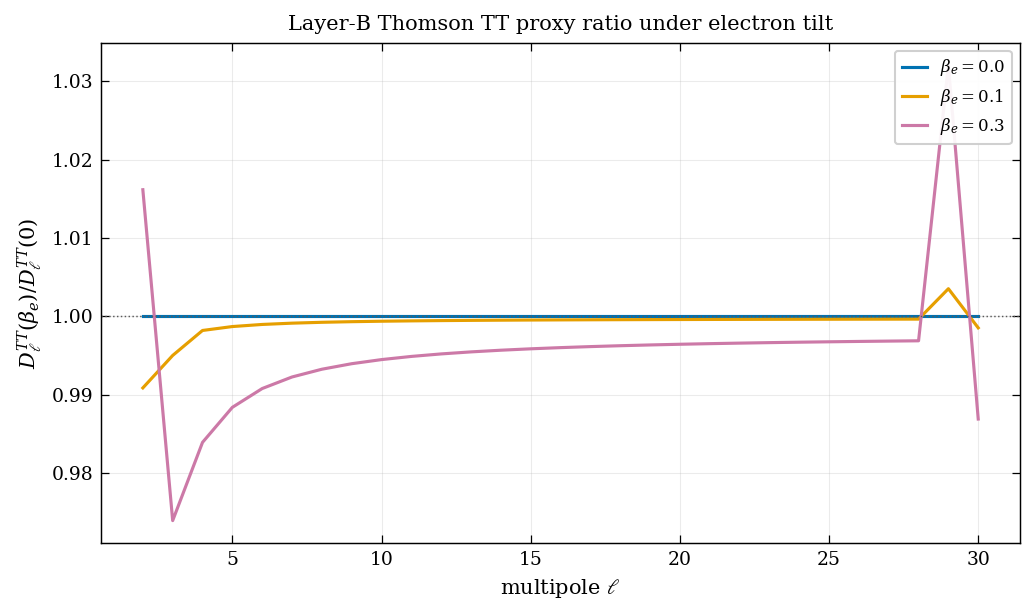
\includegraphics[width=0.82\linewidth]{figures/physics_gallery/10_collision_and_visibility/04_thomson_beta_sweep_Dl.png}
\caption{FB-4.1 gallery plot: Layer-B Thomson TT proxy ratio for
$\beta_e \in \{0,0.1,0.3\}$ on the shared PSTF seed tower.}
\label{fig:fb41-gallery}
\end{figure}

Numerically, the seeded Layer-B TT proxy remains close to the
orthogonal kernel, with the largest departures at the lowest
multipoles and percent-level excursions over
$2 \le \ell \le 30$ in Figure~\ref{fig:fb41-gallery}.  The
non-negotiable invariant is the exact $\beta_e = 0$ reduction to
the LB-4 operator, which is checked with
\texttt{np.array\_equal} in
\texttt{htt/bass/collision/test\_fb41\_tilted\_thomson\_skeleton.py}.


\subsection{FB-4.2: tilted line-of-sight $E \leftrightarrow B$ mixing}

In the same axisymmetric seed, the leading same-$\ell$
polarisation rotation is written as
\begin{equation}\label{eq:fb42-eb}
\tilde E_\ell
=
E_\ell - \frac{6\beta_e}{\ell+1} B_\ell,
\qquad
\tilde B_\ell
=
B_\ell + \frac{6\beta_e}{\ell+1} E_\ell,
\end{equation}
which makes the orthogonal Bianchi-I floor manifest:
if $B_\ell = 0$ and $\beta_e = 0$, no $B$-mode source is
generated.  Equation~(\ref{eq:fb42-eb}) is the collision-side
counterpart of the frame-change discussion in
\cite{Challinor2000} and of the Bianchi-polarisation morphology
analysed by Pontzen \& Challinor~\cite{Pontzen2011}.

\begin{figure}[h]
\centering
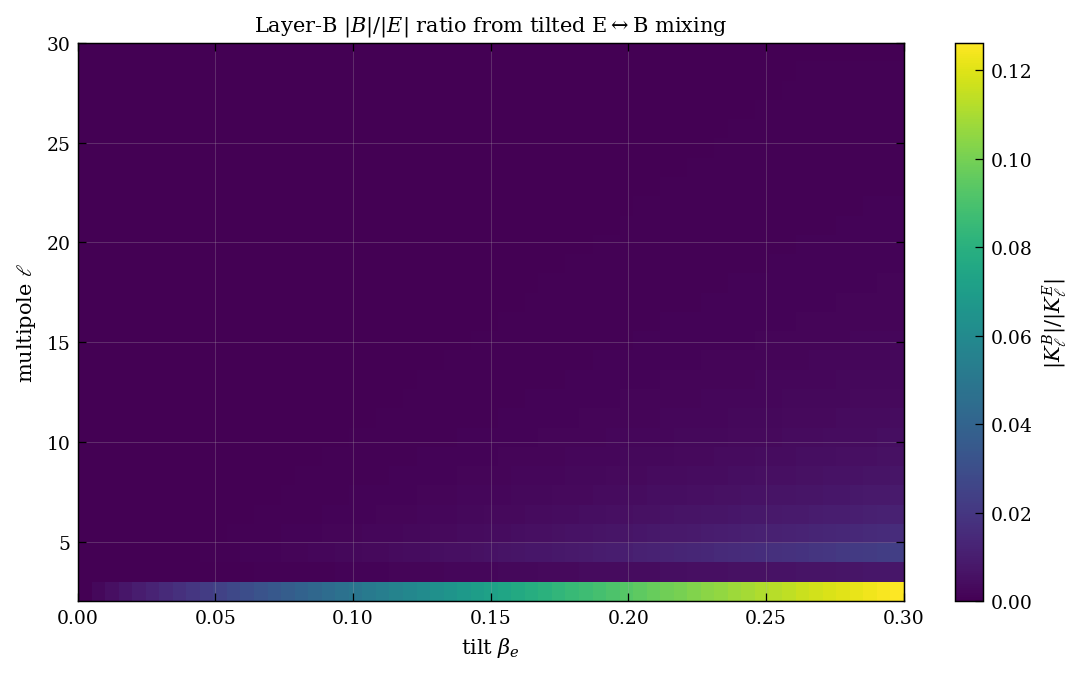
\includegraphics[width=0.82\linewidth]{figures/physics_gallery/10_collision_and_visibility/05_bb_from_tilted_lens_e.png}
\caption{FB-4.2 gallery plot: Layer-B $|B|/|E|$ ratio on the
tilted collision seed over $0 \le \beta_e \le 0.3$ and
$2 \le \ell \le 30$.}
\label{fig:fb42-gallery}
\end{figure}

Figure~\ref{fig:fb42-gallery} shows that the generated $B$ power
is concentrated in the lowest multipoles and grows monotonically
with $\beta_e$, while the exact $\beta_e = 0$ floor remains zero.
The numerical regression in
\texttt{htt/bass/collision/test\_fb42\_eb\_mixing\_skeleton.py}
verifies both the byte-identical $E$-mode reduction and the
appearance of non-zero $B$ from a pure $E$ input once the line of
sight is tilted.


% ============================================================
% ============================================================
\section{The nonperturbative $\Teff$ regime}
\label{sec:nonperturbative}
% ============================================================
% ============================================================

Our goal in this section is to delineate the domain
of validity of the $\Teff$ reduction, connect it to the
invariant manifold theory of kinetic equations, and
outline the solver programme that extends the framework
to the nonperturbative regime.  The material here is
programmatic: it describes the mathematical structure
and the planned implementation, not completed
calculations.  All claims in this section carry the
status label \textsc{Not Established} unless otherwise
noted.


% ============================================================
\subsection{Validity domain}
\label{sec:validity-domain}
% ============================================================

The $\Teff$ reduction is an exact representation of the
distribution function when the tangency diagnostic
$D_{s,\geq 2} = 0$ (Eq.~\ref{eq:D-diagnostic}), and a
controlled approximation when $D_{s,\geq 2}$ is small.
The validity domain is the region of parameter space
in which $D_{s,\geq 2}$ remains below the threshold
$\varepsilon_{\rm thr}$ set by the target observable
accuracy.

For the scalar-amplitude pipeline, the relevant
parameter space is $(\Sigstd, \beta, \Omega_K)$, and
the validity domain is determined by two conditions.
The first is the anisotropy smallness:
$|\Theta^{(s)}_{A_\ell}| \ll 1$ for all $\ell \geq 1$,
which ensures that the $\Theta^4$ moment map
(Section~\ref{sec:moment-map}) is well-approximated
by its leading-order expansion.  The second is the
collision-rate condition: for Thomson-coupled species
($\gamma$), the tight-coupling approximation
$\dot{\tau} \gg H$ suppresses the photon multipoles
above $\ell = 1$, keeping $D_{\gamma,\geq 2}$ small;
for free-streaming species ($\nu$), the tangency
diagnostic vanishes exactly because there is no collision
source to drive the distribution off the $\Teff$
manifold.

The validity domain extends to
$\Sigstd \lesssim 10^{-3}$, beyond which the
nonlinear corrections (Section~\ref{sec:comprehensive})
exceed $1\%$ and the linearised hierarchy
(Section~\ref{sec:bianchi-quad}) loses accuracy.  The
Phase~1.0 solver validates linearity ($D_2 \propto
\Sigma^2$ with spread $< 0.1\%$) over four decades
from $\Sigma^2 = 10^{-12}$ to $10^{-6}$
(Section~\ref{sec:solver-linearity}).  For the
observationally relevant range
$\Sigstd \lesssim 10^{-5}$ (the MES bound), the
$\Teff$ reduction is deep within the linear regime.


% ============================================================
\subsection{Connection to invariant manifold theory}
\label{sec:invariant-manifold}
% ============================================================

The $\Teff$ manifold of
Definition~\ref{def:species-Teff} has a natural
interpretation in the language of the Gorban--Karlin
invariant manifold programme
(Gorban \& Karlin~\cite{GorbanKarlin2005}).  The
connection, though not previously articulated in the
cosmological literature, is structurally exact and
provides rigorous foundations for the tangency
diagnostic and the upgrade policy.


\paragraph{The slow invariant manifold.}

The Gorban--Karlin framework constructs a
finite-dimensional submanifold $\Omega$ of the
infinite-dimensional space of distribution functions,
parameterised by macroscopic fields, such that
$\Omega$ is positively invariant under the kinetic
dynamics and attracts nearby trajectories.  The
central diagnostic is the \emph{defect of invariance}:
\begin{equation}\label{eq:defect-invariance}
\Delta = (1 - P)\, J(f)\,,
\end{equation}
where $J(f) = df/dt$ is the kinetic vector field and
$P$ projects onto the tangent space $T_f \Omega$.
The manifold is exactly invariant when $\Delta = 0$;
otherwise, $|\Delta|$ measures the transverse component
of the dynamics that the manifold fails to capture.


\paragraph{Identification with the $\Teff$ diagnostic.}

The per-species tangency diagnostic $D_{s,\geq 2}$
(Eq.~\ref{eq:D-diagnostic}) is the $\Teff$-specific
realisation of the Gorban--Karlin defect of invariance.
To see this, note that the $\Teff$ manifold
$\mathcal{M}_s^{\rm Teff}$ is parameterised by the
angular fields $(\Theta_s, \eta_s)$, the tangent space
$V_s = \mathrm{span}\{x_s, 1\}$
(Eq.~\ref{eq:tangent-space}) is the per-ray tangent
space of $\mathcal{M}_s^{\rm Teff}$, and the projection
$\Pi_{V_s}$ (Eq.~\ref{eq:D-diagnostic}) projects onto
$V_s$ with respect to the Fisher--entropy inner product
(Eq.~\ref{eq:fisher-inner}).  The normalised collision
field $G_{\xi,s}$
(Eq.~\ref{eq:collision-field}) plays the role of the
kinetic vector field $J(f)$ restricted to the collision
sector.  Hence
\begin{equation}\label{eq:D-equals-Delta}
D_{s,\geq 2}
= \big\| (1 - \Pi_{V_s})\, G_{\xi,s} \big\|_{*,s}
= |\Delta_s|_{*,s}\,,
\end{equation}
which is the species-resolved, per-ray defect of
invariance in the Gorban--Karlin sense.

This identification elevates the tangency diagnostic from
a heuristic quality measure to a mathematically rigorous
invariant of the closure.  The Fisher--entropy inner
product (Eq.~\ref{eq:fisher-inner}) is the cosmological
counterpart of the Gorban--Karlin thermodynamic
projector: it is the unique projection that preserves
entropy production on the $\Teff$ manifold.


\paragraph{The tight-coupling regime as a Chapman--Enskog
expansion.}

The tight-coupling approximation used in standard CMB
codes (and in the Phase~1.0 solver,
Section~\ref{sec:tight-coupling}) is functionally a
zeroth-order Chapman--Enskog expansion.  In the
Gorban--Karlin framework, the Chapman--Enskog series is
a Taylor expansion of the exact slow invariant manifold
in powers of the Knudsen number
$\mathrm{Kn} = H/\dot{\tau}$.  The zeroth-order
manifold is the two-dimensional subspace
$(\Theta_0, \Theta_1)$ on which all $\ell \geq 2$
multipoles are slaved to the monopole and dipole.  The
first-order correction adds the viscous stress
$\pi_{ab} \propto \sigma_{ab}/\dot{\tau}$, recovering
the quasi-static quadrupole
(Eq.~\ref{eq:quasi-static}).

This interpretation is well-known in kinetic theory but
has not been articulated in the cosmological Boltzmann
literature.  The connection is more than a linguistic
analogy: the spectral gap of the Thomson collision
operator (the rate $\dot{\tau}$ that damps
$\ell \geq 2$ modes) plays the same role as the BGK
collision frequency in the Gorban--Karlin analysis.  The
recombination transition ($\dot{\tau} \to 0$)
corresponds to the closure of the spectral gap---the
regime in which the slow manifold ``explodes'' and the
full hierarchy must be evolved.  The $\Teff$ formalism
provides a graceful interpolation: before recombination,
the tangency diagnostic is small and the $\Teff$ closure
is accurate; after recombination, neutrinos dominate
and their $D_{\nu,\geq 2} = 0$ exactly.


\paragraph{Spectral closure and the Kogelbauer--Karlin
programme.}

Kogelbauer \& Karlin~\cite{KogelbauerKarlin2024}
achieved exact analytical construction of the
hydrodynamic manifold for the linearised Boltzmann-BGK
equation, using spectral theory to identify the discrete
eigenvalues that separate from the essential spectrum of
the collision operator.  Their spectral temperature
$\theta(\lambda)$---encoding how the temperature degree
of freedom mixes with density and velocity within each
eigenmode---operates in the \emph{energy} direction,
decomposing the spectrum radially.  The $\Teff$ effective
temperature operates in the \emph{angular} direction,
decomposing the distribution over the sky sphere.  The
two are complementary decompositions, not competing
ones: a full spectral-angular reduction would apply the
Kogelbauer--Karlin programme at each angular multipole
$\ell$, yielding spectral temperatures $\theta_\ell$ per
mode.  This synthesis does not exist in the literature and
constitutes a natural extension of the present work.


% ============================================================
\subsection{Solver programme}
\label{sec:solver-programme}
% ============================================================

The Phase~1.0 solver of Chapter~\ref{ch:results}
operates in the linear regime
($\Sigstd \lesssim 10^{-5}$) with species-resolved
hierarchies and an analytic gravitational potential.  We
now outline the programme of extensions that pushes the
solver toward the nonperturbative regime, organised in
four phases of increasing ambition.

\emph{Phase~2.0: self-consistent Poisson.}  Replace the
analytic transfer function $\Psi(k, \eta)$
(Section~\ref{sec:flrw-oracle}) with a self-consistent
solution of the Poisson equation sourced by the
species-resolved anisotropic stress.  The target is
$|D_2^{\rm solver} - D_2^{\rm CAMB}| / D_2^{\rm CAMB}
< 2\%$, closing the $-8\%$ deviation of the Oracle~v3
(Section~\ref{sec:oracle-deviation}).  Additional
deliverables include the full neutrino hierarchy
($\ell_{\rm max,\nu} \geq 20$, replacing the current
two-moment approximation) and B-mode polarisation from
the Bianchi tensor shear.

\emph{Phase~3.0: direction-dependent $a_{\ell m}$.}
Extend the solver to produce the full
$a_{\ell m}$ spectrum, enabling pixel-level template
fitting against CMB data.  The AniCLASS
code~\cite{VicentePereiraPitrou2026} provides the
primary validation oracle for this phase.  The five
capabilities that distinguish the present solver from
AniCLASS are: species-resolved $\Teff$ spectra on Bianchi
backgrounds, the two-field neutrino treatment, the
nonperturbative regime, anisotropic recombination physics,
and the departure-parameter integration with the
BASS/HTT/MIO pipeline.

\emph{Phase~4.0: adaptive $\ell$-band hybrid.}  Implement
the three-band architecture of
Section~\ref{sec:ell-band}, with the low-$\ell$ band
using exact quadrature, the mid-$\ell$ band using the
$\Teff$ ladder with adaptive upgrading, and the
high-$\ell$ band using the standard PSTF hierarchy.  The
tangency diagnostic $D_{s,\geq 2}$ governs the band
routing at each epoch.

\emph{Phase~5.0: backreaction solver.}  Couple the
Bianchi Boltzmann solver to the Buchert spatial-averaging
framework (Section~\ref{sec:buchert-equations}),
computing the effective backreaction $\mathcal{Q}_D$ and
average curvature $\langle \mathcal{R} \rangle_D$ from
the species-resolved anisotropic stress.  The tilt
sector of the departure identity maps to the
stress-energy backreaction $\mathcal{T}_D$ in the
Buchert--Mourier--Roy~\cite{BuchertMourierRoy2020}
generalisation, providing a concrete numerical test of
the backreaction hypothesis.

The five-level error measurement hierarchy that
quantifies the solver accuracy at each phase is the
subject of Chapter~\ref{ch:error-hierarchy}.


\paragraph{Experimental timeline.}

The solver programme is designed to deliver results on a
timeline matched to the observational programme.
Phase~2.0 targets completion before Euclid~DR1
(scheduled October~2026), which will provide the first
large-area photometric catalogue for an independent
Ellis--Baldwin dipole test.  Phase~3.0 targets
completion before the Simons Observatory first-light
data ($\sim\!2027$), enabling template fitting against
ground-based high-resolution CMB polarisation.
Phases~4.0 and~5.0 are aligned with the LiteBIRD
mission ($\sim\!2033$), whose full-sky polarisation
survey will constrain $\Sigstd$ at the
$\sim\!10^{-6}$ level and directly test three or more
of the predictions derived in
Section~\ref{sec:seven-predictions}.

% === END INLINED ===

% === INLINED: figures_ch05.tex ===
% Figures for Chapter 5: The Effective Temperature Formalism
% VER05 — all figures real

\begin{figure}[t]
\centering

\includegraphics[width=\textwidth]{fig_NL_heatmap}
\caption{Nonlinear correction heatmaps in the $(\varepsilon_1, \omega/\Theta)$
  parameter plane.
  Left: shear correction factor $R_\sigma - 1$ (colour scale).
  Right: vorticity correction factor $R_\omega - 1$.
  Both corrections are below $3\%$ across the entire observational parameter
  space, confirming that the linearised MES framework is valid to better than
  $2\%$ for all scenarios considered (Section~\ref{ch:teff}).}
\label{fig:NL_heatmap}
\end{figure}

\begin{figure}[t]
\centering

\includegraphics[width=\textwidth]{fig_nonlinear_corrections}
\caption{Individual nonlinear correction factors $R_\sigma$, $R_\omega$, and
  $R_{\dot{u}}$ as functions of $\varepsilon_1$.  Shear corrections reach
  $\sim1\%$ at $\varepsilon_1 = 10^{-3}$; vorticity and acceleration
  corrections are negligible ($\lesssim 3\times 10^{-4}$) throughout the
  observational regime.  The dashed line at $\varepsilon_1 = 1.233\times10^{-3}$
  marks the CF4 inference point.}
\label{fig:nonlinear_corrections}
\end{figure}

\begin{figure}[t]
\centering

\includegraphics[width=0.85\textwidth]{fig_ell_mixing_comparison}
\caption{Doppler-boost $\ell$-mixing coefficients for $\ell_{\mathrm{out}} = 2$
  as a function of tilt rapidity $\beta$.  The dominant terms are the
  $\ell_{\mathrm{in}} = 1\to2$ and $\ell_{\mathrm{in}} = 3\to2$ couplings.
  The vertical dashed line marks $\beta_{\mathrm{CF4}} = 1.334\times10^{-3}$.
  At this value the $\ell$-mixing contamination of the quadrupole is
  $|\delta D_2| \lesssim 5\,\mu\mathrm{K}^2$.}
\label{fig:ell_mixing_comparison}
\end{figure}

\begin{figure}[t]
\centering

\includegraphics[width=0.85\textwidth]{fig_teff_moment_map}
\caption{Effective temperature moment map: contours of $\langle\Theta^4\rangle$
  in the $(A, Q)$ plane, where $A$ is the anisotropy amplitude and $Q$ the
  departure occupancy.  The star marks the VER05 posterior median.  Contours
  are equally spaced in $\log_{10}\langle\Theta^4\rangle$; the grey region
  lies below the detection threshold of the pipeline.}
\label{fig:teff_moment_map}
\end{figure}

% === END INLINED ===
